\section{Konstrukcije Ramanujanovih grafov poljubne stopnje}
Opisali bomo postopek, s katerim lahko začnemo s poljubnim dvodelnim Ramanujanovim grafom z \(n\) vozlišči in ga uporabimo za konstrukcijo dvodelnega Ramanujanovega grafa z \(2n\) vozlišči. Tako lahko začnemo s polnim dvodelnim grafom poljubne stopnje regularnosti, saj za te vemo, da so Ramanujanovi, in poiščemo večji Ramanujanov graf z enako stopnjo regularnosti. Postopek lahko nato ponavljamo induktivno in dobimo neskončno družino Ramanujanovih grafov poljubne stopnje regularnosti \cite{marcus2014interlacingfamiliesibipartite}.

\subsection{Dvodelni grafi}
Ker so dvodelni grafi v osrednjem delu tega poglavja, si poglejmo njihovo definicijo in lastnost, ki razloži, zakaj je za konstrukcijo ključno, da uporabljamo dvodelne grafe.
\begin{definicija}[Dvodelen graf]
    Graf \(G = (V, E)\) je dvodelen, če lahko množico vozlišč \(V\) razdelimo na dve disjunktni množici \(V_1\) in \(V_2\), tako da nobeni dve vozlišči iz iste množice nista sosednji.
\end{definicija}

Podobno kot smo videli, da imajo regularni grafi največjo lastno vrednost enako \(d\), lahko dokažemo, da imajo dvodelni grafi najmanjšo lastno vrednost enako \(-d\). To vrednost štejemo kot trivialno lastna vrednost in se pojavi pri vseh dvodelnih grafih.
\begin{izrek}[Najmanjša lastna vrednost]
    Naj bo \(G\) \(d\)-regularen graf. Potem je \(G\) dvodelen natanko tedaj, ko je njegova najmanjša lastna vrednost enaka \(-d\).
\end{izrek}
\begin{dokaz}
    Najprej predpostavimo, da je graf \(G\) dvodelen. Kot v definiciji razdelimo množico vozlišč na dve disjunktni množici \(V_1\) in \(V_2\).

    Izberemo vektor \(v\), ki ima vrednosti \(+1\) na mestih, ki pripadajo \(V_1\), in vrednosti \(-1\) na mestih, ki pripadajo \(V_2\). Poglejmo si vrstico sosednostne matrike, ki ustreza vozlišču iz \(V_1\). Vidimo, da ima vrstica vseh \(d\) vrednosti \(1\) na mestih, ki pripadajo \(V_2\) -- ti pa imajo v vektorju \(v\) vrednost \(-1\). Tako bo v vektorju \(v\) na takih mestih pred množenjem s sosednostno matriko vrednost \(1\), po množenju pa \(-d\). Podobno velja za vozlišča iz \(V_2\), saj so povezana samo z vozlišči v \(V_1\), kjer ima \(v\) vrednost \(+1\).

    Dokažimo še obratno; predpostavimo, da ima graf najmanjšo lastno vrednost enako \(-d\). Naj bo \(v\) lastni vektor za lastno vrednost \(-d\). Definiramo \(m = \max_i \abs{v_i}\), \(V_1=\{i \mid v_i = m\}\) in \(V_2 = \{i \mid v_i = -m\}\). Želimo dokazati, da te množici tvorita particijo kot v definiciji dvodelnih grafov.

    Opazimo, da velja 
    \begin{align*}
        -d v_i = \sum_{i\sim j} v_j.
    \end{align*}
    Če izberemo \(i\in V_1\), potem velja
    \begin{align*}
        -d m = -d v_i = \sum_{i\sim j} v_j.
    \end{align*}
    Ker so pa po absolutni vrednosti vsi \(v_j\) kvečjemu \(m\), sosedov \(i\) pa je natanko \(d\), to pomeni, da so vsi elementi vsote \(v_j\) enaki \(-m\). Iz tega pa sledi, da so vsi sosedi vozlišča \(i\) v množici \(V_2\). Obratno velja tudi, če vzamemo za \(i\) vozlišče iz \(V_2\); v tem primeru bodo vsi njegovi sosedi v \(V_1\). Ker je graf povezan, ta konstrukcija zajame vsa vozlišča, kar pomeni, da \(V_1\) in \(V_2\) tvorita particijo množice \(V\).
\end{dokaz}

Potrebujemo še zadnji izrek, ki bo razložil uporabo dvodelnih grafov v konstrukciji. V konstrukciji bomo omejili drugo največjo netrivialno lastno vrednost grafa, ne bomo pa omejili najmanjše netrivialne lastne vrednosti. Tako bi bila lahko največja netrivialna lastna vrednost po absolutni vrednosti ravno druga najmanjša lastna vrednost, ta bi pa lahko imela absolutno vrednost, ki presega mejo za Ramanujanove grafe. Dvodelni grafi pa imajo lastne vrednosti simetrične okoli ničle, torej zadošča, da omejimo samo drugo največjo lastno vrednost \cite{godsil}.

\begin{izrek}
    Če je \(G\) dvodelen graf in \(\lambda\) njegova lastna vrednost, potem je tudi \(-\lambda\) njegova lastna vrednost z enako večkratnostjo.
\end{izrek}
\begin{dokaz}
    Naj bo \(G\) dvodelen graf z particijo vozlišč \(V_1\) in \(V_2\) in naj bo \(v\) njegov lastni vektor za lastno vrednost \(\lambda\). Definirajmo \(w\) kot kandidatni lastni vektor za lastno vrednost \(-\lambda\). Vektor definiramo kot
    \begin{align*}
        w_i = \begin{cases}
                  v_i,  & i\in V_1 \\
                  -v_i, & i\in V_2
              \end{cases}
    \end{align*}
    Ker je \(v\) lastni vektor velja
    \begin{align*}
        \lambda v_i = \sum_{j\sim i} v_j.
    \end{align*}
    Vsi sosedi vozlišč iz \(V_1\) pa so v \(V_2\) in obratno, zato imajo v \(w\) pripadajoči elementi obraten predznak. Ta predznak lahko izpostavimo in zapišemo
    \begin{align*}
        -\lambda w_i = \sum_{j\sim i} w_j.
    \end{align*}
\end{dokaz}

\subsection{Dvig grafa}
Konstrukcija, ki jo bomo uporabili za konstrukcijo večjega Ramanujanovega grafa se imenuje dvig, oziroma v našem primeru, 2-dvig. Idejno 2-dvig grafa \(G\) tvori nov graf, ki ima dvakrat več vozlišč in povezav, te povezave pa so izbrane tako, da ohranimo določene lastnosti grafa. Vsako vozlišče \(v\) bo imelo v dvigu dve kopiji, \(v_1\) in \(v_2\), če pa imamo povezavo \(u\sim v\) v prvotnem grafu, ima dvig dve novi povezavi, ki povežeta \(v_1\) in \(v_2\) z \(u_1\) in \(u_2\) (ni pa določeno, ali je povezan \(v_1\sim u_1\) ali \(v_1\sim u_2\)). Pomembno je, da na ta način ohranimo stopnjo regularnosti grafa.

\begin{definicija}[2-dvig grafa]
    Naj bo \(G = (V, E)\) graf. Rečemo, da je \(G'= (V', E')\) 2-dvig grafa \(G\), če je \(V' = V + V\) (vsaj do izomorfizma natančno), za vsako povezavo \(u\sim v\) v \(G\) pa imamo v \(E'\) ali povezavi \(\{\iota_1(v)\sim \iota_1(u), \iota_2(v)\sim \iota_2(u)\}\) (povezavi prvega tipa) ali povezavi \(\{\iota_1(v)\sim \iota_2(u), \iota_2(v)\sim \iota_1(u)\}\) (povezavi drugega tipa). Drugih povezav v \(E'\) ni.
\end{definicija}

Posebej poudarimo, da \(2\)-dvig grafa ni nujno povezan. Če v dvigu uporabimo izključno povezave prvega tipa, potem dobimo disjunktno unijo dveh kopij prvotnega grafa. Če pa uporabljamo izključno povezave drugega tipa, dvig imenujemo \emph{dvojni krov} grafa. Za nas ni pomembno, vendar je zanimivo, da je konstrukcija dvodelnih Ramanujanovih grafov poljubne stopnje regularnosti lažja kot konstrukcija takih Ramanujanovih grafov, ki niso dvodelni; dvojni krov grafa bo namreč vedno dvodelen, dvojni krov nedvodelnega Ramanujanovega grafa pa bo spet Ramanujanov.

Ime izvira iz teorije kategorij. Homomorfizmi grafov preslikajo vozlišča v vozlišča in povezave v povezave. Enostavno lahko definiramo projekcijo iz \(2\)-dviga \(\pi: G'\to G\) z \(\iota_i(v)\mapsto v\), prav tako pa \(\iota_i(u)\sim\iota_j(v)\mapsto u\sim v\) za \(i, j\in \{1,2\}\). Poljuben homomorfizem \(\phi: H\to G\) lahko faktoriziramo preko \(\pi\). Vsako preslikavo povezav \(\phi\) lahko razumemo kot kompozitum dveh preslikav; najprej \(\phi'\), ki preslika \(u\sim v\) v \(\iota_i(\phi(u)) \sim \iota_j(\phi(v))\) (za ustrezno izbiro \(i\) in \(j\)) in projekcije \(\pi\). Tako lahko vsak homomorfizem \(\phi: H\to G\) zapišemo kot \(\phi = \pi\circ \phi'\) in kategorično bi bil \(\phi'\) dvig preslikave \(\phi\) na \(G'\).

\begin{definicija}[Značenje dviga]
    Značenje grafa \(G = (V, E)\) je preslikava \(s: E\to \{-1, +1\}\). Če imamo povezave oštevilčene od \(1\) do \(m\), lahko značenje definiramo kot vektor \(s\in \{-1, +1\}^m\).

    Značenje, ki pripada \(2\)-dvigu \(G'\) grafa \(G\), je preslikava \(s': E \to \{-1, +1\}\), kjer \(u\sim v \mapsto 1\), če povezavi \(u\sim v\) v dvigu pripada povezava prvega tipa, in \(-1\), če pripada povezava drugega tipa.
\end{definicija}

Iz definicije sledi, da vsako značenje enolično definira \(2\)-dvig grafa.

Sedaj lahko definiramo sosednostno matriko glede na značenje grafa. Ta bo na ničelnih vrednostih enaka navadni sosednostni matriki, kjer pa je v sosednostni matriki \(1\), bo v značeni sosednostni matriki vrednost, ki jo definira značenje.

\begin{definicija}[Značena sosednostna matrika]
    Naj bo \(G = (V, E)\) graf in \(s: E\to \{-1, +1\}\) značenje grafa. Značena sosednostna matrika \(A_s\) je \(\abs{V}\times \abs{V}\) matrika, ki ima na mestu \((u,v)\) vrednost \(0\), če \((u,v)\notin E\), in vrednost \(s(u\sim v)\), če \((u,v)\in E\).
\end{definicija}

Ta definicija ima presenetljive posledice, saj lastne vrednosti sosednostne matrike grafa in lastne vrednosti značene sosednostne matrike za značenje, ki pripada dvigu, natanko določajo lastne vrednosti dviga \cite{bilu2004constructingexpandergraphs2lifts}.
\begin{izrek}[Lastne vrednosti dviga]
    Naj bo \(G\) graf, \(G'\) njegov \(2\)-dvig in \(s\) značenje, ki pripada \(G'\). Potem so lastne vrednosti \(G'\) enake uniji lastnih vrednosti \(G\) in lastnih vrednosti \(A_s\) (skupaj z večkratnostjo).
\end{izrek}
\begin{dokaz}
    Povezave grafa razdelimo na dva dela; na povezave, ki v dvigu postanejo povezave prvega tipa, in na povezave, ki postanejo povezave drugega tipa
    \begin{align*}
        E_1 = s^{-1}(1) &  & E_2 = s^{-1}(-1).
    \end{align*}
    Ti dve podmnožici definirata podgrafa \((V, E_1)\) in \((V, E_2)\) grafa \(G\). Z \(A_1\) in \(A_2\) označimo njuni sosednostni matriki, torej velja \(A = A_1 + A_2\) in \(A_s = A_1 - A_2\).

    Vozlišča \(G'\) sestavljajo dve kopiji vozlišč iz \(G\). Če vozlišča uredimo zaporedno (torej najprej vsa vozlišča prve kopije in nato vsa vozlišča druge kopije), lahko napišemo sosednostno matriko dviga \(G'\) kot
    \begin{align*}
        A' = \begin{bmatrix}
                 A_1 & A_2 \\
                 A_2 & A_1
             \end{bmatrix}.
    \end{align*}

    Sedaj lahko uganemo lastne vektorje. Če je \(\lambda\) lastna vrednost \(A\) za lastni vektor \(v\), potem je \((v, v)\) lastni vektor za lastno vrednost \(\lambda\) matrike \(A'\). Podobno, če je \(\mu\) lastna vrednost \(A_s\) za lastni vektor \(u\), potem je \((u, -u)\) lastni vektor za lastno vrednost \(\mu\) matrike \(A'\). Če izračunamo skalarni produkt, vidimo, da so vsi lastni vektorji pravokotni med seboj, torej tvorijo bazo lastnih vektorjev in smo poiskali vse lastne vrednosti matrike \(A'\).
\end{dokaz}
Seveda iz izreka tudi sledi, da je \(2\)-dvig dvodelnega \(d\)-regularnega grafa spet dvodelen \(d\)-regularen graf, saj ohrani lastne vrednosti \(d\) in \(-d\).

\subsection{Prirejanja v grafih}
% Matching [in graph theory]
Prirejanja v grafu opisujejo, kako lahko izbiramo povezave v grafu tako, da si niso med seboj incidenčne. Število vseh možnih prirejanj določene velikosti bomo uporabili za definicijo polinoma prirejanja. Ta polinom pa ima dve ključni lastnosti, ki sta pomembni za konstrukcijo: njegove ničle znamo omejiti in polinom znamo povezati s karakteristično funkcijo značene sosednostne matrike. Na ta način lahko omejimo lastne vrednosti značene sosednostne matrike. Od prej pa že vemo, da lastne vrednosti značene sosednostne matrike določajo lastne vrednosti dviga. Na ta način bomo lahko omejili lastne vrednosti dviga in s tem dobili Ramanujanove grafe.

Da poenostavimo izražanje, označimo \(n=\abs{V}\).

\begin{definicija}[Prirejanje]
    Prirejanje velikosti \(i\) v grafu \(G\) je množica povezav \(M\subseteq E\) z \(\abs{M} = i\), za katero velja, da si nobeni dve povezavi ne delita vozlišča.

    Število vseh prirejanj velikosti \(i\) v grafu \(G\) označimo z \(m_i(G)\).
\end{definicija}

\begin{definicija}[Polinom prirejanja]
    Polinom prirejanja grafa \(G\) je
    \begin{align*}
        \mu_G(x) = \sum_{i\geq 0} (-1)^i m_i(G) x^{n-2i}.
    \end{align*}
\end{definicija}

% https://math.berkeley.edu/~nikhil/courses/270/lec1.pdf ali pa njegov source, Theory of Monomer-Dimer Systems
% v 2. viru stran 11
Dokazi lastnosti polinoma prirejanja se običajno dokazujejo z indukcijo po številu vozlišč v grafu. Poglejmo si izrek, ki nam omogoči to indukcijo.
\begin{izrek}[Rekurzivna definicija polinoma prirejanja]
    Za poljubno vozlišče \(v\) v grafu \(G\) polinom prirejanja zadošča rekurzivni zvezi
    \begin{align*}
        \mu_G(x) = x \mu_{G-\{v\}}(x) - \sum_{u\sim v} \mu_{G-\{u, v\}}(x).
    \end{align*}
    Če je \(G\) prazen graf, pa velja \(\mu_G(x) = 1\).
\end{izrek}
\begin{dokaz}
    Oglejmo si poljubno prirejanje v grafu \(G\). Če vozlišče \(v\) ni incidenčno nobeni povezavi v prirejanju, potem je to prirejanje šteto v \(m_i(G)\) in \(m_i({G-\{v\}})\). V nasprotnem primeru pa ima prirejanje povezavo \(u\sim v\). Potem je prirejanje brez te povezave šteto v \(m_{i-1}({G-\{u, v\}})\). Seveda velja tudi obratno in tako dobimo rekurzivno zvezo
    \begin{align*}
        m_i(G) = m_i({G-\{v\}}) + \sum_{u\sim v} m_{i-1}({G-\{u, v\}}).
    \end{align*}
    Sedaj to zvezo vstavimo v definicijo polinoma prirejanja.
    \begin{align*}
        \mu_G(x) & = \sum_{i\geq 0} (-1)^i m_i x^{n-2i}                                                                                             \\
                 & = \sum_{i\geq 0} (-1)^i \left( m_i({G-\{v\}}) + \sum_{u\sim v} m_{i-1}({G-\{u, v\}}) \right) x^{n-2i}                            \\
    \end{align*}
    Izraz poenostavimo in vanj vnesemo definicijo polinoma prirejanja manjšega grafa.
    \begin{align*}
        \mu_G(x) & = \sum_{i\geq 0} (-1)^i m_i({G-\{v\}}) x\cdot x^{(n-1)-2i} + \sum_{u\sim v} \sum_{i\geq 0} (-1)^i m_{i-1}({G-\{u, v\}}) x^{n-2i} \\
                 & = x \mu_{G-\{v\}}(x) + \sum_{u\sim v} \sum_{i \geq -1} -(-1)^i m_{i}(G-\{u, v\}) x^{(x-2)-2i}
    \end{align*}
    Upoštevamo, da je \(m_{-1} = 0\) in poenostavimo do konca.
    \begin{align*}
        \mu_G(x) & = x \mu_{G-\{v\}}(x) + \sum_{u\sim v} \sum_{i \geq 0} -(-1)^i m_{i}(G-\{u, v\}) x^{(x-2)-2i} \\
                 & = x \mu_{G-\{v\}}(x) - \sum_{u\sim v} \mu_{G-\{u, v\}}(x)
    \end{align*}
\end{dokaz}

Prva pomembna lastnost polinoma prirejanja je, da znamo omejiti njegove ničle, torej da so vse ničle po absolutni vrednosti manjše od neke konstante. Da to dokažemo, pa si moramo najprej ogledati prepletene družine polinomov. Dva polinoma z realnimi ničlami sta prepletena, če se ničle enega nahajajo med ničlami drugega in obratno. Pokazali bomo, da je polinom prirejanja grafa prepleten s polinomom prirejanja istega grafa z odstranjenim vozliščem.

\begin{definicija}[Prepletena polinoma]\label{prepletena-polinoma}
    Naj bosta \(n\) in \(m\) naravni števili z \(n=m\) ali \(n=m+1\). Naj bosta \(p(x) = C_1 \prod_{i=1}^n (x-\lambda_i)\) in \(q(x) = C_2 \prod_{i=1}^m (x-\nu_i)\) polinoma z realnimi ničlami \(\lambda_1 \leq \lambda_2 \leq \cdots \leq \lambda_n\) in \(\nu_1 \leq \nu_2 \leq \cdots \leq \nu_m\). V primeru \(n=m\) rečemo, da polinom \(q\) prepleta polinom \(p\), če velja
    \begin{align*}
        \nu_1 \leq \lambda_1 \leq \nu_2 \leq \lambda_2 \leq \cdots \leq \nu_n \leq \lambda_n.
    \end{align*}
    Če pa je \(n=m+1\), rečemo, da polinom \(q\) prepleta polinom \(p\), če velja
    \begin{align*}
        \lambda_1 \leq \nu_1 \leq \lambda_2 \leq \nu_2 \leq \cdots \leq \lambda_m \leq \nu_m \leq \lambda_{m+1}.
    \end{align*}
    Če so vse neenakost stroge, rečemo, da polinom \(q\) strogo prepleta polinom \(p\).
    % Manjši polinom prepleta večjega
\end{definicija}

\begin{izrek}
    Za polinom prirejanja \(\mu_G\) veljajo dve lastnosti:
    \begin{enumerate}
        \item Vse ničle polinoma \(\mu_G\) so med seboj različne in realne.
        \item Za poljubno vozlišče \(v\) grafa \(G\) polinom \(\mu_{G-\{v\}}\) strogo prepleta polinom \(\mu_G\).
    \end{enumerate}
\end{izrek}
\begin{dokaz}
    Dokaz bo potekal po indukciji. Predpostavimo, da za vsak graf \(H\) z manj kot \(n\) vozlišči velja, da ima polinom prirejanja realne ničle, ki so med seboj različne, in da za vsako vozlišče \(v\in H\) polinom \(\mu_{H-\{v\}}\) strogo prepleta polinom \(\mu_H\).

    Naj bo \(v\in G\) in naj bodo \(\lambda_1 < \cdots < \lambda_{n-1}\) ničle polinoma \(\mu_{G-\{v\}}\). Po indukciji za poljubno vozlišče \(u\in G-\{v\}\) polinom \(\mu_{G-\{v, u\}}\) strogo prepleta polinom \(\mu_{G-\{v\}}\). Polinomi prirejanja so monični, torej zavzemajo le pozitivne vrednosti desno od njihove največje ničle. Po definiciji prepletanja je \(\lambda_{n-1}\) večja od največje ničle \(\mu_{G-\{v, u\}}\), torej velja \(\mu_{G-\{v, u\}}(\lambda_{n-1}) > 0\). Dodatno, vsak interval \((\lambda_i, \lambda_{i+1})\) vsebuje natanko eno ničlo \(\mu_{G-\{v, u\}}\), torej vemo, kakšne predznake ima \(\mu_{G-\{v, u\}}\) na vseh ničlah \(\lambda_i\) -- največja ničla je pozitivna, druga največja negativna, nato spet pozitivna in tako naprej. Tako za poljuben \(u\neq v\) velja
    \begin{align*}
        \sgn\left({\mu_{G-\{v, u\}}(\lambda_i)}\right) = (-1)^{i-(n-1)},
    \end{align*}
    iz česar sledi
    \begin{align*}
        \sgn\left({\sum_{u\sim v} \mu_{G-\{u, v\}}(\lambda_i)}\right) = (-1)^{i - (n-1)}.
    \end{align*}

    Sedaj lahko uporabimo rekurzivno definicijo \(\mu_G\), da si pogledamo predznake \(\mu_G\) na ničlah \(\lambda_i\).
    \begin{align*}
        \mu_G(\lambda_i) = \lambda_i \mu_{G-\{v\}}(\lambda_i) - \sum_{u\sim v} \mu_{G-\{u, v\}}(\lambda_i) \\
        \sgn\left({\mu_G(\lambda_i)}\right) = 0 - (-1)^{i-(n-1)} (\lambda_i)
    \end{align*}
    Ker ima torej \(\mu_G\) različne predznake na \(\lambda_i\) in \(\lambda_{i+1}\), je med njima ničla. To nam zagotovi \(n-2\) različnih ničel. Ker je \(\mu_G\) moničen (torej gre spet proti \(+\infty\), ko gre \(x\to \infty\)) in \(\mu_G(\lambda_{n-1}) < 0\), obstaja še ena ničla polinoma \(\mu_G\), ki je večja od \(\lambda_{n-1}\). Podoben argument velja za ničlo, manjšo od \(\lambda_1\), torej ima \(\mu_G\) natanko \(n\) različnih ničel.
\end{dokaz}

Nadaljujemo z izrekom, ki nam bo omejil ničle polinoma prirejanja. Ta rezultat spet poteka v dveh korakih. Najprej bomo pokazali, da so ničle polinoma prirejanja grafa omejene z lastnimi vrednostmi ustreznega drevesa. Nato bomo pokazali, da so lastne vrednosti tega drevesa tudi omejene in sicer ravno z konstanto \(2\sqrt{d-1}\) -- enako konstanto, kot v definiciji Ramanujanovih grafov. Ta izrek poudari dodatno pomembnost vrednosti \(2\sqrt{d-1}\), saj omejuje spektralni radij drevesa; neskončno \(d\)-regularno drevo je univerzalni krov vsakega \(d\)-regularnega grafa, spektralni radij univerzalnega krova pa je ravno \(2\sqrt{d-1}\). Ramanujanovi grafi imajo torej vse netrivialne lastne vrednosti zajete v spektralnem radiju svojega univerzalnega krova \cite{hoory}.

\begin{definicija}[Drevo poti]
    Naj bo \(G=(V, E)\) graf. Drevo poti grafa \(G\) z izhodiščem v \(v\) je graf \(T_v(G)\), katerega vozlišča predstavljajo poti v grafu \(G\), ki se začnejo v \(v\) in ne vsebujejo nobenega vozlišča dvakrat, dve vozlišči pa sta povezani, če je pot za eno izmed vozlišč enaka kot pot za drugo vozlišče, le skrajšana za en korak.
\end{definicija}
\begin{primer}\hspace{0em}\vspace{1em}
    Za graf \(G\) vzamemo graf na sliki \ref{fig:grafnasliki12}.
    % TikZ for the graph on the left
    \begin{figure}[t]
        \centering
        \begin{tikzpicture}[node distance=1.5cm and 1cm, every node/.style={draw, circle}]
            % Nodes
            \node (a) {a};
            \node[above right=of a] (b) {b};
            \node[below right=of a] (c) {c};
            \node[below right=of b] (d) {d};
            \node[below right=of c] (e) {e};

            % Edges
            \draw (a) -- (b);
            \draw (a) -- (c);
            \draw (b) -- (d);
            \draw (c) -- (d);
            \draw (c) -- (e);
        \end{tikzpicture}
        \caption{Graf \(G\)}
        \label{fig:grafnasliki12}
    \end{figure}
    Potem je njegov graf poti \(T_a(G)\) prikazan na sliki \ref{fig:grafnasliki13}.

    % TikZ for the paths on the right
    \begin{figure}[H]
        \centering
        \begin{tikzpicture}[node distance=1.5cm and 1.5cm]
            % Nodes
            \node (a) {a};
            \node[above right=of a] (ab) {ab};
            \node[below right=of a] (ac) {ac};
            \node[right=of ab] (abd) {abd};
            \node[right=of abd] (abdc) {abdc};
            \node[right=of abdc] (abdce) {abdce};
            \node[right=of ac] (acd) {acd};
            \node[right=of acd] (acdb) {acdb};
            \node[below right=of acd] (ace) {ace};

            % Edges
            \draw (a) -- (ab);
            \draw (a) -- (ac);
            \draw (ab) -- (abd);
            \draw (abd) -- (abdc);
            \draw (abdc) -- (abdce);
            \draw (ac) -- (acd);
            \draw (acd) -- (acdb);
            \draw (acd) -- (ace);
        \end{tikzpicture}
        \caption{Drevo poti \(T_a(G)\)}
        \label{fig:grafnasliki13}
    \end{figure}
\end{primer}

\begin{lema}\label{lemarekurzpathdrevesa}
    Za vsak graf \(G\) in vsako vozlišče \(v\) velja
    \begin{align*}
        \frac{\mu_G(x)}{\mu_{G-\{v\}}(x)} = \frac{\mu_{T_v(G)}(x)}{\mu_{T_v(G)-\{v\}}(x)}.
    \end{align*}
\end{lema}
\begin{dokaz}
    Dokaz bo potekal po indukciji na številu vozlišč v grafu \(G\). Enostavno je preveriti, da izrek velja na vseh grafih z manj kot tremi vozlišči. Predpostavimo torej, da velja na vseh grafih z manj vozlišč, kot jih ima \(G\).

    Sedaj razpišemo levo stran enačbe z uporabo rekurzivne definicije \(\mu\):

    \begin{align*}
        \frac{\mu_G(x)}{\mu_{G-\{v\}}(x)} & = \frac{x \mu_{G-\{v\}}(x) - \sum_{u\sim v}\mu_{G-\{u, v\}(x)}}{\mu_{G-\{v\}}(x)} \\
                                          & = x - \sum_{u\sim v}\frac{\mu_{G-\{u, v\}(x)}}{\mu_{G-\{v\}}(x)}.
    \end{align*}
    V izrazu v vsoti lahko opazimo recipročno trditev izreka za graf \(G-\{v\}\). Na tem izrazu lahko uporabimo indukcijsko predpostavko.
    \begin{align}\label{lemamatching}
        x - \sum_{u\sim v}\frac{\mu_{T_u(G-\{v\}) - \{u\}}(x)}{\mu_{T_u(G-\{v\})}(x)}
    \end{align}
    Če drevesu \(T_v(G)\) odstranimo korensko vozlišče \(v\), dobimo disjunktno unijo dreves \(T_u(G-\{v\})\) za vsak \(u\sim v\). To lahko zapišemo kot
    \begin{align*}
        T_v(G) - \{v\} = \bigcup_{u\sim v} T_u(G-\{v\}), \\
        T_u(G - \{v\}) - \{u\} = \bigcup_{w\sim u, w\neq v} T_w(G-\{u, v\}).
    \end{align*}
    Spomnimo se, da koeficienti polinoma prirejanja štejejo število prirejanj. Če je graf nepovezan, kot je v primeru zgornje disjunktne unije, lahko prirejanja v vsaki komponenti izberemo neodvisno. Na primer, če ima graf dve komponenti in želimo poiskati prirejanje velikosti \(j\), lahko poiščemo vsa prirejanja velikosti \(i\) v prvi komponenti in vsa prirejanja velikosti \(j-i\) v drugi komponenti. Dobljeni števili zmnožimo, nato pa seštejemo za vse možne vrednosti \(i\). Opazimo, da to ravno ustreza množenju polinomov prirejanja! Seveda to velja v splošnem in lahko zapišemo
    \begin{align*}
        \mu_{T_v(G) - \{v\}}(x) = \prod_{u\sim v} \mu_{T_u(G-\{v\}) - \{u\}}(x).
    \end{align*}

    Z \(vu\) poimenujemo vozlišče v \(T_v(G)\), ki predstavlja pot od \(v\) do \(u\). Drevo \(T_v(G) - \{v\} - \{vu\}\) kot prej razpišemo kot unijo vseh dreves poti, ki se začnejo v sosedih \(v\). Nato iz te unije vzamemo drevo s korenom \(vu\) in tudi tega spremenimo v unijo, da dobimo
    \begin{align*}
        T_v(G) - \{v\} - \{vu\} & = \left(\bigcup_{w\sim v, w\neq u} T_w(G-\{v\})\right) \cup \left(\bigcup_{w\sim u, w\neq v} T_w(G-\{v,u\})\right) \\
                                & = \left(\bigcup_{w\sim v, w\neq u} T_w(G-\{v\})\right) \cup (T_u(G-\{v\}) - \{u\})
    \end{align*}
    Spet so ta drevesa disjunktna, torej velja
    \begin{align*}
        \mu_{T_v(G) - \{v\} - \{vu\}}(x) = \left(\prod_{w\sim v, w\neq u} \mu_{T_w(G-\{v\})}(x)\right) \mu_{T_u(G-\{v\}) - \{u\}}(x) \\
        \mu_{T_u(G-\{v\}) - \{u\}}(x) = \frac{\mu_{T_v(G) - \{v\} - \{vu\}}(x)}{\prod_{w\sim v, w\neq u} \mu_{T_w(G-\{v\})}(x)}
    \end{align*}
    Zdaj lahko dobljeni produkt vstavimo v izraz \ref{lemamatching}.
    \begin{align*}
        \frac{\mu_G(x)}{\mu_{G-\{v\}}(x)} & =x - \sum_{u\sim v}\frac{\mu_{T_v(G) - \{v\} - \{vu\}}(x)}{(\prod_{w\sim v, w\neq u} \mu_{T_w(G-\{v\})}(x))(\mu_{T_u(G-\{v\})}(x))} \\
                                          & = x - \sum_{u\sim v}\frac{\mu_{T_v(G) - \{v\} - \{vu\}}(x)}{(\prod_{w\sim v} \mu_{T_w(G-\{v\})}(x))}                                \\
                                          & = x - \sum_{u\sim v}\frac{\mu_{T_v(G) - \{v\} - \{vu\}}(x)}{\mu_{T_v(G-\{v\})}(x)}                                                  \\
                                          & = \frac{x \mu_{T_v(G-\{v\})}(x) - \sum_{u\sim v} \mu_{T_v(G) - \{v\} - \{vu\}}(x)}{\mu_{T_v(G-\{v\})}(x)}
    \end{align*}
    Da zaključimo dokaz, le uporabimo rekurzivno definicijo polinoma prirejanja.
    \begin{align*}
        \frac{\mu_G(x)}{\mu_{G-\{v\}}(x)} = \frac{\mu_{T_v(G)}(x)}{\mu_{T_v(G-\{v\})}(x)}
    \end{align*}
\end{dokaz}

To lemo uporabimo, da pokažemo, da so ničle polinoma prirejanja nekega grafa tudi ničle polinoma prirejanja njegovega grafa poti.
% https://www.cs.yale.edu/homes/spielman/561/lect26-18.pdf

\begin{izrek}
    Za poljubno vozlišče \(v\in G\) polinom \(\mu_G\) deli polinom \(\mu_{T_v(G)}\).
\end{izrek}
\begin{dokaz}
    Dokazujemo z indukcijo po številu vozlišč grafa \(G\). Trditev enostavno preverimo za grafe z manj kot tremi vozlišči. Predpostavimo torej, da izrek velja za vse grafe z manj vozlišči kot jih ima \(G\). Za poljubno povezavo \(u\sim v\) potem velja, da \(\mu_{G-\{v\}}\) deli \(\mu_{T_u(G-\{v\})}\).

    Ker velja
    \begin{align*}
        T_v(G) - \{v\} = \bigcup_{w\sim v} T_w(G-\{v\}), \\
        \mu_{T_v(G) - \{v\}} = \prod_{w\sim v} \mu_{T_w(G-\{v\})},
    \end{align*}
    sledi, da \(\mu_{T_u(G-\{v\})}\) deli \(\mu_{T_v(G) - \{v\}}\). Torej tudi \(\mu_{G-\{v\}}\) deli \(\mu_{T_v(G) - \{v\}}\) in izraz
    \begin{align*}
        \frac{\mu_{T_v(G) - \{v\}}(x)}{\mu_{G-\{v\}}(x)}
    \end{align*}
    je polinom v \(x\). Po lemi \ref{lemarekurzpathdrevesa} je enak izrazu
    \begin{align*}
        \frac{\mu_{T_v(G)}(x)}{\mu_{G}(x)},
    \end{align*}
    torej \(\mu_G\) deli \(\mu_{T_v(G)}\).
\end{dokaz}

Trditev izreka lahko izrazimo tudi drugače: vse ničle polinoma prirejanja grafa \(G\) so tudi ničle polinoma prirejanja njegovega grafa poti. Če torej znamo omejiti ničle polinoma prirejanja grafa poti, lahko omejimo tudi ničle polinoma prirejanja grafa. Dokaz, da so te ničle res omejene, bo potekal v dveh korakih. Najprej pokažemo, da je polinom prirejanja drevesa enak njegovemu karakterističnemu polinomu, nato pa pokažemo, da so ničle tega polinoma omejene.

\begin{izrek}\label{drevo-karakteristicni}
    Če je \(T\) drevo in \(A\) njegova sosednostna matrika, potem velja:
    \begin{align*}
        \mu_T(x) = \chi_A(x).
    \end{align*}
\end{izrek}
\begin{dokaz}
    Po definiciji razpišemo karakteristični polinom in upoštevamo, da je \(A\) na diagonali ničelna.
    \begin{align*}
        \chi_A(x) & = \det(xI - A)\\
                  & = \sum_{\pi \in S_n}\sgn(\pi)x^{\abs{\{v \mid \pi(v) = v\}}}\prod_{v \mid \pi(v)\neq v}(-A)_{v,\pi(v)}
    \end{align*}

    Pokazali bomo, da k vsoti prispevajo le involucije, torej permutacije \(\pi\), za katere velja \(\pi(\pi(v)) = v\) za vsak \(v\). Če obstaja \(v\), za katerega velja \(\pi(\pi(v))\neq v\), potem ima permutacija \(\pi\) cikel dolžine \(k\geq 3\). Da je sumand, ki pripada tej permutaciji, neničelen, morajo biti vsi elementi sosednostne matrike, ki pripadajo ciklu, enaki \(1\). To bi pa pomenilo, da ima tudi graf cikel, kar pa ni mogoče, saj je \(T\) drevo.

    Involucije v grafu pa ustrezajo prirejanjem. Sestavljene so samo iz fiksnih točk in ciklov dolžine \(2\). Da to pokažemo, vzamemo neko involucijo, ki pripada neničelnemu sumandu. Ker je involucija, ima le cikle dolžine 2 in fiksne točke, vsi cikli pa pripadajo elementom, ki so neničelni v sosednostni matriki -- torej sta vozlišči povezani in vsak cikel predstavlja povezavo. V permutaciji pa ne smeta biti predstavljeni dve incidenčni povezavi, saj bi to pomenilo, da obstaja cikel dolžine več od 2. To pa je ravno definicija prirejanja. Če ima involucija \(k\) ciklov, potem jo prištejemo h koeficientu \(x^{n-2k}\), njen znak pa je \((-1)^k\) -- kar ustreza definiciji polinoma prirejanja.
\end{dokaz}

Sedaj lahko ocenimo lastne vrednosti drevesa.

\begin{izrek}\label{lastne-vrednosti-drevesa}
    Naj bo \(T\) drevo, v katerem ima vsako vozlišče stopnjo največ \(d\). Potem so vse lastne vrednosti \(T\) po absolutni vrednosti omejene z \(2\sqrt{d-1}\).
\end{izrek}
\begin{dokaz}
    Naj bo \(A\) sosednostna matrika \(T\). Vzamemo poljubno vozlišče \(v\in T\) za koren drevesa in definiramo funkcijo \(h\) na vozliščih \(T\), ki nam poda razdaljo posameznega vozlišča do korena.

    Definiramo še diagonalno matriko \(D\) z elementi
    \begin{align*}
        D_{v, v} = \sqrt{d-1}^{h(v)}.
    \end{align*}
    Matrika je seveda obrnljiva in lastne vrednosti \(A\) so enake lastnim vrednostim \(D A D^{-1}\). Matrika \(DAD^{-1}\) ima vse elemente nenegativne, torej je po izreku \ref{def-najvecja-lv} njena največja lastna vrednost manjša ali enaka njeni največji vrstični vsoti. Če torej pokažamo, da so vsote vseh vrstic manjše od \(2\sqrt{d-1}\), bomo s tem dokazali trditev. Ločimo tri primere: vrstica, ki pripadajo korenu, listom in preostalim vozliščem.

    Najprej si oglejmo vrstico matrike \(DAD^{-1}\), ki pripada korenu. Matrika \(A\) ima v tej vrstici kvečjemu \(d\) neničelnih elementov, vsak od njih pa se zmnoži z \(\sqrt{d-1}^{-1}\), ko množimo iz desne z \(D^{-1}\) in z \(1\), ko množimo z \(D\) iz leve. Torej je vsota elementov v tej vrstici kvečjemu \(d/\sqrt{d-1}\), kar je manj kot \(2\sqrt{d-1}\) za \(d\geq 2\).

    Nato si oglejmo vrstice, ki pripadajo listom. Naj bo \(v\) ta list. Ima le enega soseda, njegova višina pa je za ena manjša od višine \(v\). Ko množimo \(A\) iz desne z \(D^{-1}\), dobimo vrstico, ki ima le en element neničelen, in sicer je enak \(\sqrt{d-1}^{-h(v)+1}\). Ko to vrstico množimo iz leve z \(D\), dobimo vrstico, ki ima le en element neničeln, ta pa je \(\sqrt{d-1}^{-h(v)+1}\sqrt{d-1}^{h(v)}\) oziroma \(\sqrt{d-1}\), spet manjše od \(2\sqrt{d-1}\).

    Preostala vozlišča \(v\) imajo en element, ki ima višino manjšo za ena in kvečjemu \(d-1\) elementov, ki imajo višino večjo za ena. Torej bo po množenju z \(D^{-1}\) iz desne v vrstici en element \(\sqrt{d-1}^{-h(v)+1}\) in kvečjemu \(d-1\) elementov \(\sqrt{d-1}^{-h(v)-1}\). Ko množimo iz leve z \(D\) se vsi elementi pomnožijo z \(\sqrt{d-1}^{h(v)}\). Vsota je torej kvečjemu \(\sqrt{d-1} + (d-1)/\sqrt{d-1}\) oziroma \(2\sqrt{d-1}\).
\end{dokaz}

Zdaj, ko imamo informacije o ničlah polinoma prirejanja, lahko opišemo, kako so te ničle povezane z značeno sosednostno matriko dviga.

\begin{izrek}\label{znacenje-prirejanje}
    Za značenje \(s\) in značeno sosednostno matriko \(A_s\) naj bo \(f_s(x) = \det(xI - A_s)\) karakteristični polinom. Potem velja
    \begin{align*}
        \mathbb{E}_{s\in \{\pm 1\}^m} f_s(x) = \mu_G(x).
    \end{align*}
\end{izrek}
\begin{dokaz}
    Z \(\mathrm{Sym}(S)\) označimo množico vseh permutacij na množici \(S\) in z \(\abs{\pi}\) označimo število inverzij permutacije \(\pi\). Z \(n\) označimo število vozlišč. Determinanto najprej razpišemo kot vsoto po permutacijah \(\sigma\in \mathrm{Sym}([n])\), nato pa to vsoto spremenimo v vsoto po vseh permutacijah, ki imajo \(k\) fiksnih točk (ter seštejemo vse \(k\)). Za preglednejši zapis uvedemo oznako \(\mathrm{fix}(S) = \{\sigma \in \mathrm{Sym}([n]) \mid \forall i\in S.\, \sigma(i) = i \}\).
    \begin{align*}
        \det(xI - A_s) & = \sum_{\sigma\in \mathrm{Sym}([n])}\sgn(\sigma)\prod_{i=1}^n(xI-A_s)_{i, \sigma(i)} \\
                       & = \sum_{k=0}^n \sum_{\substack{S \subseteq [n]                                       \\ \abs{S} = k}} \sum_{\sigma \in \mathrm{fix(S)}}\sgn(\sigma)\prod_{i=1}^n(xI-A_s)_{i, \sigma(i)}\\
                       & = \sum_{k=0}^n \sum_{\substack{S \subseteq [n]                                       \\ \abs{S} = k}} \sum_{\sigma \in \mathrm{fix(S)}}\sgn(\sigma) x^{k} \prod_{i\in \overline{S}} (-A_s)_{i, \sigma(i)}\\
    \end{align*}
    Na produkt gledamo kot produkt po določenih povezavah v grafu. Iteriramo po vseh možnih vrednostih \(i\), ki niso fiksne točke permutacije. Če \((i, \sigma(i))\) ni povezava v grafu, je ta produkt enak \(0\), torej upoštevamo le tiste permutacije, za katere velja, da je \(i\) ali fiksna točka ali pa \((i, \sigma(i))\) povezava v grafu. To označimo z \(\mathrm{efix}(S) = \{\sigma \in \mathrm{fix}(S) \mid \forall i\in \overline{S}.\, (i, \sigma(i))\in E \}\).
    \begin{align*}
        \det(xI - A_s) = \sum_{k=0}^n x^{k} \sum_{\substack{S \subseteq [n] \\ \abs{S} = k}} \sum_{\sigma \in \mathrm{efix(S)}}\sgn(\sigma)  \prod_{(i, \sigma(i))\in E} (-A_s)_{i, \sigma(i)}
    \end{align*}
    Na povezavah pa je vrednost značene sosednostne matrike enaka značenju \(s\).
    \begin{align*}
        \det(xI - A_s) = \sum_{k=0}^n x^{k} \sum_{\substack{S \subseteq [n] \\ \abs{S} = k}} \sum_{\sigma \in \mathrm{efix(S)}}\sgn(\sigma)  \prod_{(i, \sigma(i))\in E} -s(i, \sigma(i))
    \end{align*}

    Zdaj si ogledamo pričakovano vrednost.
    \begin{align*}
        \mathbb{E}_{s\in \{\pm 1\}^m} \left[\det(xI - A_s)\right] & = \mathbb{E}_{s\in \{\pm 1\}^m} \left[ \sum_{k=0}^n x^{k} \sum_{\substack{S \subseteq [n] \\ \abs{S} = k}} \sum_{\sigma \in \mathrm{efix(S)}}\sgn(\sigma)  \prod_{(i, \sigma(i))\in E} -s(i, \sigma(i))\right] \\
        & = \sum_{k=0}^n x^{k} \sum_{\substack{S \subseteq [n] \\ \abs{S} = k}} \sum_{\sigma \in \mathrm{efix(S)}} \sgn(\sigma)  \mathbb{E}_{s\in \{\pm 1\}^m} \left[ \prod_{(i, \sigma(i))\in E} -s(i, \sigma(i)) \right]\\
    \end{align*}
    Najprej si oglejmo produkt \(\prod s\), za tem bomo pa izračunali prispevek negativnih predznakov in izračunali produkt \(\prod (-s)\). Ker računamo pričakovano vrednost po vseh možnih značenjih je \(\mathbb{E}[s(i,j)] = 0\). Če izberemo \((i,j)\) in \(A\subset [n]\times [n]\), kjer \((i,j) \notin A\) in \((j,i)\notin A\), potem je \(s(i,j)\) neodvisen od vseh ostalih \(s(k,l)\) (za \((k,l)\in A\)), saj lahko značenje vsakega roba izberemo neodvisno od ostalih. Torej je
    \begin{align*}
        \mathbb{E}\left[s(i,j) \prod_{(k,l)\in A} s(k,l)\right] & = \mathbb{E}[s(i,j)]\mathbb{E}\left[\prod_{(k,l)\in A} s(k,l)\right] \\
                                                                & = 0.
    \end{align*}
    To se ne zgodi v primeru \(2\)-cikla, kjer je \(\mathbb{E}(s(i,j)s(j,i)) = 1\). Torej bodo vsi produkti ničelni, razen tisti, ki jih sestavljajo samo \(2\)-cikli in fiksne točke. Kot smo že videli v dokazu izreka \ref{drevo-karakteristicni}, take permutacije predstavljajo prirejanja v grafu. Produkt bo torej \(1\), če permutacija predstavlja prirejanje in \(0\) sicer.

    Zdaj določimo še predznak sumanda. Znak permutacije je določen s številom inverzij, ki je enako številu povezav v prirejanju (vsaka inverzija predstavlja krajišča povezave). Imamo \(n-k\) vozlišč, ki so del prirejanja, torej imamo \((n-k)/{2}\) povezav. Tako je predznak \(\sgn{\sigma} = (-1)^{\frac{n-k}{2}}\). Produkt \(\prod -s\) množi sodo mnogo elementov (saj je sestavljen iz samih \(2\)-ciklov), torej se negativni predznaki \(-s\) pokrajšajo.
    \begin{align*}
        \mathbb{E}_{s\in \{\pm 1\}^m} \det(xI - A_s) & =\sum_{k=0}^n x^{k} \sum_{\substack{S \subseteq [n]        \\ \abs{S} = k}} \sum_{\sigma \in \mathrm{efix(S)}} (-1)^{\frac{n-k}{2}} \\
                                                     & =\sum_{k=0}^n x^{k} m_{\frac{n-k}{2}} (-1)^{\frac{n-k}{2}} \\
                                                     & = \sum_{i \geq 0} m_i (-1)^{i} x^{n-2i}
    \end{align*}
\end{dokaz}

Preden se lotimo glavnega dela dokaza, potrebujemo še lemo, ki opisuje ničle značenih karakterističnih polinomov.

\subsection{Realno stabilni polinomi}
Na prvi pogled je cilj tega poglavja nekoliko nenavaden. Dokazati želimo, da so, za poljubna števila \(p_1, \ldots, p_m \in [0,1]\) ničle polinoma
\begin{align*}
    \sum_{s\in \{\pm 1\}^m} \left(\prod_{\substack{(i,j) \\s(i,j)=1}} p_{i,j}\right) \left(\prod_{\substack{(i,j)\\s(i,j)=-1}} (1- p_{i,j})\right) f_s(x)
\end{align*}
realne. Iz te trditve bomo kasneje lahko sklepali, da so polinomi \(f_s\) prepleteni, podobno, kot so bili prepleteni polinomi prirejanja. Prepletene družine pa nosijo veliko informacij o ničlah funkcij, ki jih tvorijo.

Za dokaz potrebujemo še nekaj definicij in lem. Želimo posplošiti pojem realne ničle na polinome z več spremenljivkami. Če imamo polinom v eni spremenljivki z realnimi koeficienti, lahko ničle delimo na realne in na kompleksne (z neničelno imaginarno komponento). Realne ničle so lahko samostojne, kompleksne pa vedno prihajajo v konjugiranih parih. Lahko torej rečemo, da ima polinom same realne ničle, če nima nobene ničle, ki ima imaginarno komponento večjo od nič (saj iz tega sledi, da nima tudi nobenih z imaginarno komponento manjšo od nič). Posledica, da so vse ničle strogo realne, ne velja v večjih dimenzijah, bomo pa karakterizacijo vseeno uporabili za definicijo realno stabilnih polinomov.
\begin{definicija}[Realno stabilen polinom]
    Polinom \(f\in \mathbb R[z_1, \ldots, z_n]\) je realno stabilen, če je ničelen polinom ali pa velja
    \begin{align*}
        \left(\forall i.\, \Im(z_i) > 0\right) \implies f(z_1, \ldots, z_n) \neq 0.
    \end{align*}
\end{definicija}
V literaturi se pogosto uporabljajo tudi drugačne definicije. V našem primeru ničle ne smejo biti na določenem kvadrantu, lahko bi pa definirali, da so vse ničle na kakšni kompleksni polravnini ali kateremkoli drugem kvadrantu. Definicije imajo skupno, da prepovedujejo ničle na določenem delu kompleksne ravnine, ker pa lahko ta del preoblikujemo s pomočjo Möbiusove transformacije, lahko vsako trditev, ki uporablja eno definicijo, preoblikujemo v trditev, ki uporablja drugo \cite{mckenzie}.

Zdaj si lahko ogledamo družino realno stabilnih polinomov, ki jo bomo potrebovali v našem izreku \cite{JuliusPetter}.
\begin{izrek}\label{matrike-realnostabilna}
    Za \(1\leq j \leq n\) naj bodo \(A_j\) pozitivno semidefinitne matrike. Potem je polinom
    \begin{align*}
        f(z_1, \ldots, z_n) = \det\left(\sum_{j=1}^n z_j A_j\right)
    \end{align*}
    realno stabilen.
\end{izrek}
Za dokaz izreka potrebujemo Hurwitzev izrek \cite{freitag1}.
\begin{izrek}[Hurwitzev izrek]\label{hurwitz}
    Naj bo \(D\) domena v \(\mathbb C^n\) in \((f_k)_{k=1}^\infty\) zaporedje analitičnih funkcij na \(D\) brez ničel, ki konvergirajo enakomerno proti funkciji \(f\) na kompaktnih podmnožicah \(D\). Potem \(f\) ali nima ničle na \(D\) ali pa je identična \(0\).
\end{izrek}
Hurwitzevega izreka ne bomo dokazali, saj je standarden rezultat iz kompleksne analize. Lahko pa si ogledamo dokaz izreka \ref{matrike-realnostabilna}.
\begin{dokaz}
    Zaradi Hurwitzevega izreka lahko predpostavimo, da so vse \(A_j\) pozitivno definitne. Definiramo si funkcijo \(z: \mathbb C\to \mathbb C\) kot \(z(t) = \alpha + \lambda t\), kjer je \(\alpha\in \mathbb R^n\) in \(\lambda \in \mathbb R_+^n\). Lastnost te funkcije je, da če pa ima katerakoli komponenta slike \(\Im(z(t))>0\), potem tudi \(\Im(t)>0\). Lahko pa dobimo poljuben element iz \(\mathbb C_+^n\), za primerno izbiro \(\alpha\), \(\lambda\) in \(t\); torej, če poiščemo vse ničle \(f(z(t))\) in ugotovimo, da nobena nima \(\Im(t)>0\), potem je \(f\) realno stabilen.

    Matrika \(P = \sum_j \lambda_j A_j\) je pozitivno definitna, torej je obrnljiva in ima kvadraten koren, ki je tudi sam definiten. Definiramo si še \(H = \sum_j \alpha_j A_j\). Zdaj razpišemo \(f(z(t))\).
    \begin{align*}
        f(z(t)) & = \det\left(\sum_{j=1}^n (\alpha_j + \lambda_j t) A_j\right) \\
                & = \det\left(\sum_{j=1}^n \alpha_j A_j + t\sum_{j=1}^n \lambda_j A_j\right)
    \end{align*}
    V izraz vstavimo definicijo \(H\) in \(P\).
    \begin{align*}
        f(z(t))  = \det\left(H+ tP\right)
    \end{align*}
    Iz determinante izpostavimo kvadratni koren \(P^{\frac12}\).
    \begin{align*}
        f(z(t)) = \det\left(P^{1/2}\right)\det\left(P^{-1/2}HP^{-1/2} + tI\right) \det\left(P^{1/2}\right)
    \end{align*}
    Ker sta matriki \(H\) in \(P^{-1/2}\) definitni je tudi \(P^{-1/2}HP^{-1/2}\) definiten. Torej je izraz enak skalarnemu večkratniku karakterističnega polinoma pozitivno definitne matrike (za skalar \(\det(P)\)). Ta pa ima same realne ničle, torej je \(\Im(t)=0\).
\end{dokaz}

Sedaj potrebujemo še nekaj načinov, kako konstruiramo nove realno stabilne polinome iz že znanih. Očitno je, da je produkt dveh realno stabilnih polinomov spet realno stabilen. Imamo pa še dve drugi konstrukciji, ki ju bomo potrebovali \cite{wagner-multivariate}.
\begin{izrek}[Specializacija realno stabilnih polinomov]
    Naj bo \(f(z_1, \ldots, z_n)\) realno stabilen polinom. Potem je za poljuben \(a\in \mathbb C\) z \(\Im(a)\geq 0\) polinom \(g(z_2, \ldots, z_n) = f(a, z_2, \ldots, z_n)\) realno stabilen.
\end{izrek}
\begin{dokaz}
    Rezultat je očiten, če je \(Im(a) > 0\). Za \(\Im(a) = 0\) pa uporabimo Hurwitzev izrek. Naj bo torej \(a\in \mathbb R\). Za domeno vzamemo
    \begin{align*}
        D=\{(z_2,\ldots,z_n) \in \mathbb C^{n-1}\mid \forall 2\leq j \leq n.\, \Im(z_j)> 0\}.
    \end{align*}
    Nato za \(a_k = a + i 2^{-k}\) definiramo zaporedje polinomov
    \begin{align*}
        g_k(z_2, \ldots, z_n) = f(a_k, z_2, \ldots, z_n).
    \end{align*}
    Ti polinomi seveda konvergirajo lokalno enakomerno proti \(g(z_2, \ldots, z_n)\) in so realno stabilni. Po Hurwitzevem izreku je \(g\) realno stabilen.
\end{dokaz}
Če za konstanto vzamemo \(a=1\), vidimo, da so tudi polinomi oblike \(\det(B + \sum A_i z_i)\) realno stabilni.
Posebej bomo potrebovali primer, kjer je \(a = 0\). Tako definiramo operator \(Z_j\), da vzame realno stabilen polinom v \(n\) spremenljivkah, zamenja spremenljivko \(z_j\) s konstanto \(0\) in vrne realno stabilen polinom v \(n-1\) spremenljivkah.

Potrebovali bomo še način, kako dobimo nov realno stabilen polinom preko odvodov. Z \(\partial_j\) označimo delni odvod po \(j\)-ti spremenljivki \cite{Borcea_2010}.
\begin{izrek}[Odvajanje realno stabilnih polinomov]
    Naj bo \(f(z_1, \ldots, z_n)\) realno stabilen polinom, \(p, q\in \mathbb R\) in \(1\leq i, j \leq n\). Potem je polinom
    \begin{align*}
        (1+p\partial_i + q\partial_j)f
    \end{align*}
    realno stabilen.
\end{izrek}
Izreka ne bomo dokazali, ga pa potrebujemo v nadaljevanju.

Da se lotimo izrekov, ki zagotavljajo, da imajo določeni polinomi realne ničle, potrebujemo še dve manjši lemi. Prva je standardni rezultat iz linearne algebre, ki nam pomaga izračunati determinanto cite{matrix-determinant-lemma}, z drugo pa izračunamo rezultat zgoraj definiranih operatorjev na določenih polinomih, dobljenih iz determinant.
\begin{lema}\label{matrix-det-lemma}
    Če je \(A\in \mathbb C^{n\times n}\) obrnljiva matrika in \(u, v \in \mathbb C^n\) vektorja, potem velja
    \begin{align*}
        \det(A + uv^\top) = \det(A) (1 + v^\top A^{-1} u).
    \end{align*}
\end{lema}
\begin{dokaz}
    Najprej predpostavimo \(A=I\). Velja enakost
    \begin{align*}
        \begin{bmatrix}
            I      & 0 \\
            v^\top & 1
        \end{bmatrix}
        \begin{bmatrix}
            I + uv^\top & u \\
            0           & 1
        \end{bmatrix}
        \begin{bmatrix}
            I       & 0 \\
            -v^\top & 1
        \end{bmatrix}
        =
        \begin{bmatrix}
            I & u            \\
            0 & 1 + v^\top u
        \end{bmatrix}
    \end{align*}
    Ker je determinanta odvisna le od diagonalnih blokov, dobimo želeno enakost.

    Sedaj posplošimo na primer za splošen \(A\). Ker je \(A+uv^\top= A(I + A^{-1}uv^\top)\) je
    \begin{align*}
        \det(A + uv^\top) & = \det(A) \det(I + (A^{-1}u)v^\top) \\
                          & = \det(A) (1 + v^\top A^{-1} u).
    \end{align*}
\end{dokaz}

\begin{lema}\label{zizj-odvod-determinante}
    Naj bo \(A\) obrnljiva matrika, \(a,b\) vektorja in \(p\in [0,1]\) število. Potem velja
    \begin{align*}
        Z_iZ_j(1+p\partial_i + (1-p)\partial_j)\det(A + z_i aa^\top+ z_j bb^\top) \\
        = p\det(A + aa^\top) + (1-p)\det(A+bb^\top).
    \end{align*}
\end{lema}
\begin{dokaz}
    S prejšno lemo izračunamo odvod determinante.
    \begin{align*}
        \partial_i \det(A + z_i aa^\top +z_j bb^\top) & =\partial_i \left(\det(A + z_j bb^\top) (1+ z_i a^\top (A + z_j bb^\top)^{-1} a)\right) \\
                                                      & = \det(A + z_j bb^\top) a^\top (A + z_j bb^\top)^{-1} a                                 \\
        \partial_j \det(A + z_i aa^\top +z_j bb^\top) & = \det(A + z_i aa^\top) b^\top (A + z_i aa^\top)^{-1} b
    \end{align*}
    tako lahko izračunamo rezultat operatorja \((1+p\partial_i + (1-p)\partial_j)\).
    \begin{align*}
         & (1+p\partial_i + (1-p)\partial_j)\det(A + z_i aa^\top + z_j bb^\top) = \\
         & = \det(A + z_i aa^\top + z_j bb^\top)                                  \\
         & + p\det(A + z_j bb^\top) a^\top (A + z_j bb^\top)^{-1} a               \\
         & + (1-p)\det(A + z_i aa^\top) b^\top (A + z_i aa^\top)^{-1} b
    \end{align*}
    Sedaj pa uporabimo operatorja \(Z_i\) in \(Z_j\), ki vse \(z_i\) in \(z_j\) zamenjata z \(0\).
    \begin{align*}
         & Z_iZ_j(1+p\partial_i + (1-p)\partial_j)\det(A + z_i aa^\top+ z_j bb^\top) = \\
         & =\det(A) + p\det(A) a^\top A^{-1} a + (1-p)\det(A) b^\top A^{-1} b          \\
         & = p \det(A)(1+ a^\top A^{-1}a) + (1-p)\det(A)(1+b^\top A^{-1} b)
    \end{align*}
    Sedaj lahko dvakrat ponovno uporabimo prejšno lemo, da zaključimo dokaz
    \begin{align*}
        p \det(A + aa^\top) + (1-p)\det(A+bb^\top).
    \end{align*}
\end{dokaz}

Zdaj si ogledamo še zadnja dva izreka. Oba opisujeta, da ima določena družina polinomov same realne ničle, kar pa je ravno cilj trenutnega poglavja.
\begin{izrek}\label{realne-nicle-velik-polinom-1}
    Naj bodo \(a_1, \ldots, a_m\) in \(b_1, \ldots, b_m\) vektorji v \(\mathbb R^n\), \(p_1,\ldots, p_m \in [0,1]\) in \(A\) pozitivno definitna matrika. Potem ima polinom
    \begin{align*}
        P(x) = \sum_{S\subseteq [m]} \left(\prod_{i\in S} p_i\right)\left(\prod_{i\notin S} \left(1-p_i\right)\right) \det\left(xI + A + \sum_{i\in S} a_i a_i^\top + \sum_{i\notin S} b_i b_i^\top\right)
    \end{align*}
    same realne ničle.
\end{izrek}
\begin{dokaz}
    Definiramo polinom
    \begin{align*}
        Q(x, u_1, \ldots, u_m, v_1, \ldots, v_m) = \det\left(xI + A + \sum_{i=1}^m u_i a_i a_i^\top + \sum_{i=1}^m v_i b_i b_i^\top\right).
    \end{align*}
    Kot vemo iz leme \ref{matrike-realnostabilna} je ta polinom realno stabilen.

    Definiramo si \(T_i = 1+p_i\partial_{1+i} + (1-p_i)\partial_{1+m+i}\) (odvajamo po spremenljivki \(u_i\) in \(v_i\) v \(Q\)). Sedaj želimo dokazati, da
    \begin{align*}
        P(x) = \left(\prod_{i=1}^m Z_{1+i}Z_{1+m+i}T_i\right)Q(x, u_1, \ldots, u_m, v_1, \ldots, v_m).
    \end{align*}
    To pokažemo tako, da dokažemo, da je izraz
    \begin{align*}
        \left(\prod_{i=1}^k Z_{1+i}Z_{1+m+i}T_i\right)Q(x, u_1, \ldots, u_m, v_1, \ldots, v_m)
    \end{align*}
    enak izrazu
    \begin{align*}
        \sum_{S\subseteq [k]} & \left(\prod_{i\in S} p_i\right)\left(\prod_{i\in [k]\setminus S} \left(1-p_i\right)\right) \\
                              & \cdot\det\left(xI + A + \sum_{i\in S} a_i a_i^\top + \sum_{i\in [k]\setminus S} b_i b_i^\top + \sum_{i>k} \left( u_i a_i a_i^\top + v_i b_i b_i^\top\right)\right)
    \end{align*}
    za vsak \(k\). Dokaza se lotimo induktivno po \(k\). Za \(k=0\) je izraz enak po definiciji. Za induktivni korak pa uporabimo lemo \ref{zizj-odvod-determinante}. Oglejmo si le prvi korak, ostali sledijo analogno.
    \begin{align*}
         & Z_{1+i} Z_{1+m+i} T_i Q \\
         & =Z_{1+i} Z_{1+m+i} T_i \det\left(xI + A + \sum_{j=1}^m u_j a_j a_j^\top + \sum_{j=1}^m v_j b_j b_j^\top\right)
    \end{align*}
    Iz vsote izločimo sumande za indeks \(j=1\).
    \begin{align*}
         & =Z_{1+i} Z_{1+m+i} T_i \det\left(\left(xI + A + \sum_{j=2}^m u_j a_j a_j^\top + \sum_{j=2}^m v_j b_j b_j^\top\right) + u_1 a_1 a_1^\top + v_1 b_1 b_1^\top\right)
    \end{align*}
    Na izrazu uporabimo lemo \ref{zizj-odvod-determinante}.
    \begin{align*}
         & = p_i \det\left(xI + A + \sum_{j=2}^m u_j a_j a_j^\top + \sum_{j=2}^m v_j b_j b_j^\top + a_1 a_1^\top\right) \\
         & + (1-p_i) \det\left(xI + A + \sum_{j=2}^m u_j a_j a_j^\top + \sum_{j=2}^m v_j b_j b_j^\top + b_1 b_1^\top\right)
    \end{align*}
    Rezultat lahko zapišemo v obliki, ki je enaka željenemu izrazu.
    \begin{align*}
        \sum_{S\subseteq \{1\}} & \left(\prod_{i\in S} p_i\right)\left(\prod_{i\in \{1\}\setminus S} \left(1-p_i\right)\right)  \\
                                & \cdot \det\left(xI + A + \sum_{i > 1} (u_i a_i a_i^\top + v_i b_i b_i^\top) + \sum_{i\in S}a_ia_i^\top \sum_{i\in \{1\}\setminus S} b_i b_i^\top\right)
    \end{align*}
    Naslednje korake izvedemo enako, saj lahko operator prinesemo znotraj vsote in produktov. V zadnjem koraku, \(k=m\) dobimo željeno enakost. Vemo pa, da operatorji \(Z_i\) in \(T_i\) ohranjajo realno stabilnost, torej, ker je \(Q\) realno stabilen, je tudi \(P\) realno stabilen. Ker pa ima le eno spremenljivko in realne koeficiente, so njegove kompleksne ničle prisotne v konjungiranih parih; če ima kakšno ničlo z \(\Im(z_0)<0\), ima tudi ničlo z \(\Im(z_0)>0\), kar pa je v protislovju z realno stabilnostjo. Torej so vse ničle realne.
\end{dokaz}

Sedaj izrek uporabimo, da zaključimo poglavje, in dokažemo trditev iz začetka poglavja o realni stabilnosti.

\begin{izrek}\label{nicle-prepletenih-so-realne}
    Za vsako povezavo \((i,j)\) grafa naj bo \(p_{i,j}\in [0,1]\). Potem ima polinom
    \begin{align*}
        \sum_{s\in \{\pm 1\}^m} \left(\prod_{\substack{(i,j) \\s(i,j)=1}} p_{i,j}\right) \left(\prod_{\substack{(i,j)\\s(i,j)=-1}} (1- p_{i,j})\right) f_s(x)
    \end{align*}
    same realne ničle.
\end{izrek}
\begin{dokaz}
    Najprej razpišemo \(f_s\) po definiciji
    \begin{align*}
        \sum_{s\in \{\pm 1\}^m} \left(\prod_{\substack{(i,j) \\s(i,j)=1}} p_{i,j}\right) \left(\prod_{\substack{(i,j)\\s(i,j)=-1}} (1- p_{i,j})\right) \det(xI - A_s).
    \end{align*}
    Seveda, če ima polinom \(f(x)\) realne ničle, ima tudi zamaknjen polinom \(f(x+d)\) (za poljuben \(d\in \mathbb R\)) same realne ničle. Za \(d\) izberemo maksimalno stopnjo vozlišča v grafu (oziroma največji seštevek absolutnih vrednosti elementov vrstic \(A_s\)). Tako si ogledamo polinom
    \begin{align*}
        \sum_{s\in \{\pm 1\}^m} \left(\prod_{\substack{(i,j) \\s(i,j)=1}} p_{i,j}\right) \left(\prod_{\substack{(i,j)\\s(i,j)=-1}} (1- p_{i,j})\right) \det(xI + dI - A_s).
    \end{align*}
    Strukturo tega polinoma želimo zapisati tako, da lahko uporabimo trditev prejšnega izreka. Za to si moramo ogledati strukturo matrike \(dI - A_s\). Za vsako povezavo \((i,j)\in E\) v grafu definiramo matriki
    \begin{align*}
        L_{i,j}^1 = (e_i-e_j)(e_i-e_j)^\top, \\
        L_{i,j}^{-1} = (e_i+e_j)(e_i+e_j)^\top.
    \end{align*}
    Obe matriki imata vrednost \(1\) na mestih \((i,i)\) in \((j,j)\). Prva matrika ima vrednost \(-1\) na mestih \((i,j)\) in \((j,i)\), druga pa ima tudi tam vrednost \(1\). Če seštejemo matrike za vsa vozlišča, bodo na diagonali ravno stopnje vozlišč, s pravilno izbiro pa lahko opišemo tudi značenje povezav. Tako lahko zapišemo
    \begin{align*}
        dI - A_s = \sum_{(i,j)\in E} L_{i,j}^{s(i,j)} + D,
    \end{align*}
    kjer je \(D\) diagonalna matrika z nenegativnimi elementi (saj je \(d\) največja stopnja vozlišča). Torej je \(D\) pozitivno semidefinitna matrika. Če sedaj izberemo \(a_{i,j} = (e_i-e_j)\) in \(b_{i,j} = (e_i+e_j)\) lahko uporabimo izrek \ref{realne-nicle-velik-polinom-1}, da dokažemo, da so vse ničle realne.
\end{dokaz}

\subsection{Prepletena značenja}
Prepletene polinome smo že srečali v dokazih za prirejanja v grafih. Izkazalo se je, da polinom prirejanja grafa prepleta polinom prirejanja istega grafa z dodanim vozliščem. Sedaj si bomo ogledali drugačno družino prepletenih polinomov, in sicer \(\{f_s\}_{s\in \{\pm 1\}^m}\). Pokazali bomo, da je družina prepletena in da imajo prepletene družine polinomov vsaj en polinom, ki ima največjo ničlo manjšo od največje ničle pričakovane vrednosti cele družine. Ker pa zaradi izreka \ref{znacenje-prirejanje} že poznamo dobro oceno za pričakovano vrednost, bo to pokazalo obstoj nekega polinoma, ki ima največjo ničlo dovolj majhno. To pa je ravno pogoj, da je graf Ramanujanov, kot bomo povzeli po zaključku vseh potrebnih dokazov.

Najprej posplošimo definicijo \ref{prepletena-polinoma} prepletenih polinomov na družino polinomov.
\begin{definicija}[Skupno prepletanje]
    Polinomi \(f_1, \ldots, f_k\) imajo skupno prepletanje, če obstaja polinom \(g\), ki prepleta vse polinome \(f_i\).
\end{definicija}
\begin{definicija}[Prepletena družina]\label{prepletena-druzina}
    Naj bodo \(S_1, \ldots, S_m\) končne množice in za poljuben element \((s_1, \ldots, s_m)\in S_1\times \ldots \times S_m\) naj bo \(f_{s_1, \ldots, s_m}\) polinom stopnje \(n\) z realnimi ničlami in pozitivnim vodilnim koeficientom.

    Za \(0\leq k<m\) definiramo
    \begin{align*}
        f_{(s_1, \ldots, s_k)}(x) = \sum_{(s_{k+1}, \ldots, s_m)\in S_{k+1}\times \ldots \times S_m} f_{s_1, \ldots, s_m}(x).
    \end{align*}

    Množica \(\{f_{s_1,\ldots, s_m}\}_{s_1,\ldots, s_m\in S_1\times \ldots \times S_m}\) tvori prepleteno družino, če imajo za vsak \(0\leq k<m-1\) in \(s_1, \ldots, s_k\in S_1\times \ldots \times S_k\) polinomi \(\{f_{(s_1, \ldots, s_k, t)}\}_{t\in S_{k+1}}\)  skupno prepletanje.
\end{definicija}
V definiciji nam indeksi fiksirajo določene parametre, seštevamo pa po vseh možnih nefiksiranih parametrih. V skrajnosti, \(f_{()}\) sešteje kar vse polinome v družini.

Za nas bo zanimiv primer, ko so vsi \(S_i=\{-1, +1\}\), posamezni \(s_i\) pa predstavljajo značenje določenega robova. Polinom \(f_{s_1, \ldots, s_m}\) bo predstavljal značeni karakteristični polinom za značenje \((s_1,\ldots, s_m) \in \{\pm 1\}^m\). Primer \(f_{()}\) sešteje vsa možna značenja, torej je do skalarja natančno enak pričakovani vrednosti vseh značenih karakterističnih polinomov (seveda ima tudi enake ničle). Družina značenih karakterističnih polinomov bo pa prepletena, če, ne glede na to kako definiramo značenje robova (imamo pa fiksirano značenje za robove, ki imajo manjši indeks), obstaja nek polinom, ki prepleta pričakovani polinom po nefiksiranih spremenljivkah. To pa omejuje koliko se lahko spremenijo ničle, saj morajo biti ničle prepletenega polinoma med ničlami pričakovanega polinoma.

Najprej bomo dokazali, da značeni karakteristični polinomi res tvorijo prepleteno družino. Za to potrebujemo drugačno karakterizacijo skupnih prepletanj \cite{DEDIEU1992269}.
\begin{izrek}\label{konveksne-kombinacije-prepletenih}
    Naj bodo \(f_1, \ldots, f_k\) polinomi v eni spremenljivki enake stopnje s pozitivnimi vodilnimi koeficienti. Potem imajo polinomi skupno prepletanje natanko takrat, ko ima \(\sum_{i=1}^k \lambda_i f_i\) realne ničle za vse konveksne kombinacije \(\lambda_i\) (torej \(\lambda_i\geq 0\) in \(\sum_{i=1}^k \lambda_i=1\)).
\end{izrek}
Dokazali bomo le za nas pomembno smer, da imajo polinomi skupno prepletanje, če ima vsaka njihova konveksna kombinacija realne ničle. Zaradi enostavnosti predpostavimo tudi, da je \(k=2\). Dokaz poteka enako tudi v primeru \(k>2\).
\begin{dokaz}
    Naj bosta \(f =  k_1 \prod_{i=1}^n (x-a_i)\) in \(g =  k_2 \prod_{i=1}^n (x-b_i)\) polinoma. Ker je primer \(n=1\) trivialen, predpostavimo \(n\geq2\). Kot v trditvi izreka predpostavimo, da ima polinom \(h = \lambda f + (1-\lambda) g\) realne ničle za poljubno vrednost \(\lambda\). Za začetek še predpostavimo splošno lego ničel: vse ničle polinomov \(f\) in \(g\) so različne.

    Polinoma imata skupno prepletanje, če obstaja polinom \(p\) stopnje \(n-1\), ki prepleta oba polinoma. To lahko enostavno karakteriziramo, če si ogledamo zaporedje ničel. Če je \(a_i < b_{i+1}\) so možne kombinacije ničel
    \begin{itemize}
        \item \(a_i < b_i < a_{i+1} < b_{i+1}\)
        \item \(a_i < b_i < b_{i+1} < a_{i+1}\)
        \item \(a_i < a_{i+1} < b_i < b_{i+1}\)
    \end{itemize}
    Podobno velja, če je \(b_i < a_{i+1}\). V prvem primeru lahko za ničlo polinoma \(p\) izberemo poljubno vrednost med \(b_{i}\) in \(a_{i+1}\), v drugem pa med \(b_i\) in \(b_{i+1}\). Če so vse ničle torej prve ali druge oblike, lahko polinom \(p\) enostavno določimo. Torej moramo dokazati le, da če so vse ničle konveksne kombinacije realne, potem ni mogoče, da si ničle \(f\) in \(g\) sledijo kot v tretjem primeru (za kateri koli \(i\)). Lažji je dokaz v kontrapozitivni obliki: dokazali bomo, da če so ničle kot v tretjem primeru ima konveksna kombinacija polinomov kompleksno ničlo.

    Predpostavimo torej, da je \(a_i < a_{i+1} < b_i < b_{i+1}\). Izberemo si najmanjši tak \(i\); s tem zagotovimo, da ne obstaja noben \(j<i\), za katerega bi veljalo \(a_i < b_j < b_i\). S to izbiro zagotovimo, da \(g\) ne spremeni predznaka med \(a_i\) in \(b_i\). Ker sta polinoma \(f\) in \(g\) monična in enake stopnje se predznaki med ničlami alternirajo enako. Recimo, če ima \(f\) med \(a_i\) in \(a_{i+1}\) pozitiven predznak, ima tudi \(g\) med \(b_i\) in \(b_{i+1}\) pozitiven predznak. To skupaj povzamemo v tabeli (kjer predpostavimo, da ima \(f(x)\) pozitiven predznak pred \(b_i\) in da je \(\varepsilon\) dovolj majhen).
    \begin{center}
        \begin{align*}
            \begin{array}{|c|c|c|c|c|c|}
                \hline
                     & (a_i - \varepsilon, a_i) & (a_i, a_{i+1}) & (a_{i+1}, b_i) & (b_i, b_{i+1}) & (b_{i+1}, b_{i+1} + \varepsilon) \\ \hline
                g(x) & +                        & +          & +          & -          & +                        \\ \hline
                f(x) & +                        & -          & +          & +          & +                        \\ \hline
            \end{array}
        \end{align*}
    \end{center}
    Torej naš \(h(x)=\lambda f(x) + (1-\lambda) g(x)\) ima za \(\lambda = 1\) ničli v \(a_i\) in \(a_{i+1}\), ko zmanjšujemo \(\lambda\) pa se njegova vrednost na intervalu \((a_i, a_{i+1})\) povečuje, saj se prištevajo same pozitivne vrednosti. Za \(\lambda=1\) ima na tem intervalu same negativne vrednosti, za \(\lambda=0\) pa same pozitivne. Vrednosti izven intervala \((a_i, a_{i+1})\) so začele pozitivne in končale pozitivne. Ker je proces zvezen v \(\lambda\) in je \(h\) za vsak \(\lambda\) polinom, to pomeni, da je za nek \(\lambda\) ničla dvojna. Če temu \(\lambda\) odštejemo še dovolj majhen \(\varepsilon>0\) dobimo kompleksno ničlo.

    Tako smo dokazali, da če so ničle \(f\) in \(g\) v nezaželeni obliki, je nekje ničla konveksne kombinacije kompleksna. Ker pa predpostavka izreka zahteva, da so vse ničle konveksne kombinacije realne, to pomeni, da so vse ničle \(f\) in \(g\) v taki obliki, da lahko izberemo ničle polinoma \(p\), ki ju prepleta.

    Rezultat v izrojenih primerih, kjer imata \(f\) ali \(g\) večkratne ničle dobimo tako, da polinoma zamaknemo za \(\varepsilon\), da odpravimo večkratne ničle, in pošljemo \(\varepsilon\to 0\). Če pa si \(f\) in \(g\) delita ničlo, torej \(f(x) = (x-a)^{m_f} f_1(x)\) in \(g(x) = (x-a)^{m_g} g_1(x)\) lahko to ničlo izpostavimo iz konveksne kombinacije in nadaljujemo kot v splošni legi. 
\end{dokaz}

V tem izreku pa vidimo nekaj zanimivega: pojem prepletenosti je povezan z obstojem realne ničle. V izreku \ref{nicle-prepletenih-so-realne} pa smo pokazali ravno, da imajo določeni polinomi realne ničle. To lahko uporabimo, da pokažemo, da značeni karakteristični polinomi tvorijo prepleteno družino.

\begin{izrek}\label{karakteristicni-so-prepleteni}
    Družina polinomov \(\{f_s\}_{s\in \{\pm 1\}^m}\) tvori prepleteno družino.
\end{izrek}
\begin{dokaz}
    Zaradi izreka \ref{konveksne-kombinacije-prepletenih} moramo le pokazati, da imajo polinomi
    \begin{align*}
        \lambda f_{s_1, \ldots s_k, 1}(x) + (1-\lambda)f_{s_1,\ldots, s_k, -1}(x)
    \end{align*}
    realne ničle za vse \(\lambda\in [0,1]\) in \(s_1, \ldots, s_k\in \{\pm 1\}\). Fiksirajmo \(s_1, \ldots, s_k\) in dokažimo, da so ničle realne.

    V izreku \ref{nicle-prepletenih-so-realne} smo pokazali, da so ničle polinoma
    \begin{align*}
        \sum_{s\in \{\pm 1\}^m} \left(\prod_{\substack{i \\s_i=1}} p_{i}\right) \left(\prod_{\substack{i\\s_i=-1}} (1- p_{i})\right) f_s(x)
    \end{align*}
    realne. Za koeficiente izberemo \(p_{k+1}=\lambda\), \(p_{k+2},\ldots, p_m=1/2\) in \(p_i = (1+s_i)/2\) za \(1\leq i\leq k\). Iz \(p_{k+1}\) dobimo koeficient \(\lambda\), ko prištevamo polinom z \(s_{k+1}=1\) in \(1-\lambda\), ko prištevamo polinom z \(s_{k+1} = -1\). Preko \(p_i = (1+s_i)/2\) poskrbimo, da ostanejo le členi, ki imajo pravilno značenje (torej, da so \(s_i\) kot smo izbrali na začetku), ostali členi pa se zmnožijo v \(0\). Nazadnje pa z \(p_i = 1/2\) ne uničimo ničesar; v vsakem seštevku bomo dobili le \((1/2)^{m-(k+2)}\), kar pa ne vpliva na ničle, saj lahko ta faktor izpostavimo. Dobimo torej 
    \begin{align*}
        \left(\frac12\right)^{m-(k+2)}\left(\lambda \sum_{s\in \{\pm 1\}^{m-(k+2)}}f_{s_1, \ldots, s_k, 1, s}(x) +(1-\lambda) \sum_{s\in \{\pm 1\}^{m-(k+2)}}f_{s_1, \ldots, s_k, -1, s}(x)\right)
    \end{align*}
    Oziroma, po definiciji,
    \begin{align*}
        \left(\frac12\right)^{m-(k+2)}(\lambda f_{s_1, \ldots, s_k, 1} + (1-\lambda)f_{s_1,\ldots, s_k, -1}(x)).
    \end{align*}
    Torej so ničle konveksne kombinacije realne in družina \(f_s\) je prepletena.
\end{dokaz}

Sedaj lahko zaključimo z zadnjim izrekom, ki bo pokazal obstoj polinoma, katerega največja ničla je dovolj majhna.

\begin{lema}\label{obstaja-nicla-manjsa}
    Naj bodo \(f_1, \ldots, f_k\) polinomi enake stopnje s pozitivnim vodilnim koeficientom in skupnim prepletanjem. Potem obstaja \(i\), za katerega ima polinom \(f_i\) največjo ničlo manjšo ali enako največji ničli polinoma \(f=\sum_{i=1}^k f_i\).
\end{lema}
\begin{dokaz}
    Naj bodo vsi polinomi stopnje \(n\) in naj polinom \(g\) prepleta vse \(f_i\). Dodatno naj bo \(\alpha_{n-1}\) največja ničla \(g\).
    
    Po definiciji prepletanja ima vsak polinom \(f_i\) največ eno ničlo, ki je večja od \(\alpha_{n-1}\). Ker polinom \(g\) prepleta vse \(f_i\) je \(f_i(\alpha_{n-1})\leq0\) za vse \(i\). Ker imajo polinomi pozitiven vodilni koeficient so za dovolj velike \(x\) pozitivni, torej je tudi njihov seštevek sčasoma pozitiven in ima ničlo \(\beta_n > \alpha_{n-1}\).

    Dokažimo zdaj s protislovjem. Naj imajo vsi polinomi največjo ničlo strogo večjo od \(\beta_n\). Potem lahko izberemo tisti \(i\), za katerega je največja ničla \(f_i\) najmanjša izmed največjih ničel vseh polinomov. Ta ničla je še vedno večja od \(\beta_n\), poimenujemo jo \(\gamma_n\). Za njo velja, da je \(f_i(\gamma_n) \leq 0\) za vse \(i\), ampak \(f(\gamma_n) > 0\). Ker pa seštevek nepozitivnih števil ne more biti pozitiven, smo v protislovju in torej obstaja neka ničla, ki je manjša ali enaka največji ničli polinoma \(f\).
\end{dokaz}

\begin{izrek}
    Obstaja značenje \(s\) za katerega je največja ničla \(f_s\) manjša od največje ničle pričakovane vrednosti \(\mathbb E_{s}(f_s)\).
\end{izrek}
\begin{dokaz}
    Družina polinomov \(\{f_s\}_{s\in\{\pm1\}^m}\) je, kot vemo iz izreka \ref{karakteristicni-so-prepleteni}, prepletena družina. Seštevek te družine je \(f_{()}\), ki ima enake ničle kot pričakovana vrednost \(\mathbb E_{s}(f_s)\) (saj sta do skalarnega večkratnika natančno enaka polinoma). Sedaj lahko induktivno določimo značenja robov.

    Začnemo z množico \(\{f_{(1)}, f_{(-1)}\}\), (spomnimo se definicije \ref{prepletena-druzina}, ki definira \(f_{(1)}\) kot seštevek vseh značenih karakterističnih polinomov, ki imajo značenje za prvi rob fiksirano na \(1\); enako seveda za \(f_{(-1)}\), ki fiksira značenje roba na \(-1\)). Polinoma imata skupno prepletanje, saj je družina \(\{f_s\}\) prepletena. Zaradi leme \ref{obstaja-nicla-manjsa} pa ima eden od njiju največjo ničlo, ki je manjša od njunega seštevka \(f_{()}\). Za \(s_1\) vzamemo značenje roba, ki ga je fiksiral ta polinom. Nato nadaljujemo induktivno z množico \(\{f_{s_1, 1}, f_{s_1, -1}\}\) in tako naprej, dokler ne določimo značenja za vse robove. Seštevek množice v vsakem koraku je polinom iz prejšnjega koraka, za katerega vemo, da ima največjo ničlo dovolj majhno. 
\end{dokaz}

\subsection{Konstrukcija}
Sedaj imamo vse potrebne izreke, da predstavimo konstrukcijo Ramanujanovih grafov.

Začnemo z dvodelnim \(d\)-regularnim Ramanujanovim grafom. Za vsak tak graf lahko poiščemo njegov \(2\)-dvig, ki ima dvakrat več vozlišč in ohranja dvodelnost. Vsakemu \(2\)-dvigu pripada značenje in ga lahko opišemo z značeno sosednostno matriko. Lastne vrednosti \(2\)-dviga so ravno unija lastnih vrednosti prvotnega grafa in lastnih vrednosti značene sosednostne matrike. Če začnemo z Ramanujanovim grafom so njegove lastne vrednosti že dovolj majhne in, da je njegov \(2\)-dvig Ramanujanov, potrebujemo le pokazati, da je največja lastna vrednost značene sosednostne matrike dovolj majhna. Največja lastna vrednost značene sosednostne matrike pa je ravno največja ničla značenega karakterističnega polinoma. Preko polinomov prirejanja smo pokazali, da je \(\mathbb E_{s}f_s(x) = \mu_G(x)\). Ker si polinomi prirejanja grafa delijo ničle z karakterističnimi polinomi dreves poti istega grafa in, ker za vsa drevesa znamo omejiti lastne vrednosti z \(2\sqrt{d-1}\), dobimo, da je največja ničla \(\mathbb E_{s}f_s(x)\) manjša od \(2\sqrt{d-1}\). Preko prepletenih družin pa smo pokazali, da obstaja neko specifično značenje, ki ima največjo ničlo karakterističnega polinoma manjšo od največje ničle \(\mathbb E_{s}f_s(x)\), torej tudi od \(2\sqrt{d-1}\). Če sedaj izberemo za novi graf \(2\)-dvig, ki pripada temu značenju, dobimo, da so vse netrivialne lastne vrednosti manjše od \(2\sqrt{d-1}\). Ker je graf dvodelen so lastne vrednosti simetrične okoli nič, torej so lastne vrednosti manjše tudi po absolutni vrednosti. To pa je ravno definicija Ramanujanovega grafa.

\begin{primer}
    Za primer si bomo ogledali konstrukcijo \(4\)-regularnih grafov. Začnemo s polnim dvodelnim grafom \(K_{4,4}\). Za tega vemo, da je Ramanujanov. Njegova sosednostnja matrika je
    \begin{align*}
        \begin{bmatrix}
            0 & 0 & 0 & 0 & 1 & 1 & 1 & 1\\
            0 & 0 & 0 & 0 & 1 & 1 & 1 & 1\\
            0 & 0 & 0 & 0 & 1 & 1 & 1 & 1\\
            0 & 0 & 0 & 0 & 1 & 1 & 1 & 1\\
            1 & 1 & 1 & 1 & 0 & 0 & 0 & 0\\
            1 & 1 & 1 & 1 & 0 & 0 & 0 & 0\\
            1 & 1 & 1 & 1 & 0 & 0 & 0 & 0\\
            1 & 1 & 1 & 1 & 0 & 0 & 0 & 0\\
    \end{bmatrix}.
    \end{align*}
    \begin{figure}[H]
        \centering
        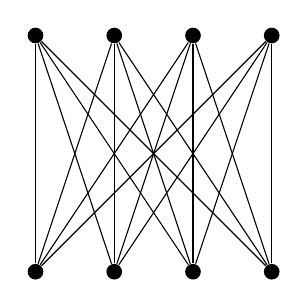
\begin{tikzpicture}[scale=1, transform shape]
          \node[circle, fill=black, inner sep=2pt] (L0) at (1.5, 0) {};
          \node[circle, fill=black, inner sep=2pt] (L1) at (0.5, 0) {};
          \node[circle, fill=black, inner sep=2pt] (L2) at (-0.5, 0) {};
          \node[circle, fill=black, inner sep=2pt] (L3) at (-1.5, 0) {};
          \node[circle, fill=black, inner sep=2pt] (R0) at (1.5, 3) {};
          \node[circle, fill=black, inner sep=2pt] (R1) at (0.5, 3) {};
          \node[circle, fill=black, inner sep=2pt] (R2) at (-0.5, 3) {};
          \node[circle, fill=black, inner sep=2pt] (R3) at (-1.5, 3) {};
          \draw (L0) -- (R0);
          \draw (L0) -- (R1);
          \draw (L0) -- (R2);
          \draw (L0) -- (R3);
          \draw (L1) -- (R0);
          \draw (L1) -- (R1);
          \draw (L1) -- (R2);
          \draw (L1) -- (R3);
          \draw (L2) -- (R0);
          \draw (L2) -- (R1);
          \draw (L2) -- (R2);
          \draw (L2) -- (R3);
          \draw (L3) -- (R0);
          \draw (L3) -- (R1);
          \draw (L3) -- (R2);
          \draw (L3) -- (R3);
        \end{tikzpicture}
    \end{figure}
    Nato izbiramo njegove \(2\)-dvige naključno, dokler ne dobimo takega, ki je Ramanujanov. Naključno izberemo dvig s sosednostnjo matriko
    \begin{align*}
        \begin{bmatrix}
            0 & 0 & 0 & 0 & 1 & 1 & 1 & 1 & 0 & 0 & 0 & 0 & 0 & 0 & 0 & 0\\
            0 & 0 & 0 & 0 & 1 & 1 & 1 & 1 & 0 & 0 & 0 & 0 & 0 & 0 & 0 & 0\\
            0 & 0 & 0 & 0 & 1 & 1 & 1 & 1 & 0 & 0 & 0 & 0 & 0 & 0 & 0 & 0\\
            0 & 0 & 0 & 0 & 1 & 1 & 1 & 0 & 0 & 0 & 0 & 0 & 0 & 0 & 0 & 1\\
            1 & 1 & 1 & 1 & 0 & 0 & 0 & 0 & 0 & 0 & 0 & 0 & 0 & 0 & 0 & 0\\
            1 & 1 & 1 & 1 & 0 & 0 & 0 & 0 & 0 & 0 & 0 & 0 & 0 & 0 & 0 & 0\\
            1 & 1 & 1 & 1 & 0 & 0 & 0 & 0 & 0 & 0 & 0 & 0 & 0 & 0 & 0 & 0\\
            1 & 1 & 1 & 0 & 0 & 0 & 0 & 0 & 0 & 0 & 0 & 1 & 0 & 0 & 0 & 0\\
            0 & 0 & 0 & 0 & 0 & 0 & 0 & 0 & 0 & 0 & 0 & 0 & 1 & 1 & 1 & 1\\
            0 & 0 & 0 & 0 & 0 & 0 & 0 & 0 & 0 & 0 & 0 & 0 & 1 & 1 & 1 & 1\\
            0 & 0 & 0 & 0 & 0 & 0 & 0 & 0 & 0 & 0 & 0 & 0 & 1 & 1 & 1 & 1\\
            0 & 0 & 0 & 0 & 0 & 0 & 0 & 1 & 0 & 0 & 0 & 0 & 1 & 1 & 1 & 0\\
            0 & 0 & 0 & 0 & 0 & 0 & 0 & 0 & 1 & 1 & 1 & 1 & 0 & 0 & 0 & 0\\
            0 & 0 & 0 & 0 & 0 & 0 & 0 & 0 & 1 & 1 & 1 & 1 & 0 & 0 & 0 & 0\\
            0 & 0 & 0 & 0 & 0 & 0 & 0 & 0 & 1 & 1 & 1 & 1 & 0 & 0 & 0 & 0\\
            0 & 0 & 0 & 1 & 0 & 0 & 0 & 0 & 1 & 1 & 1 & 0 & 0 & 0 & 0 & 0\\
    \end{bmatrix}.
    \end{align*}
    \begin{figure}[H]
        \centering
        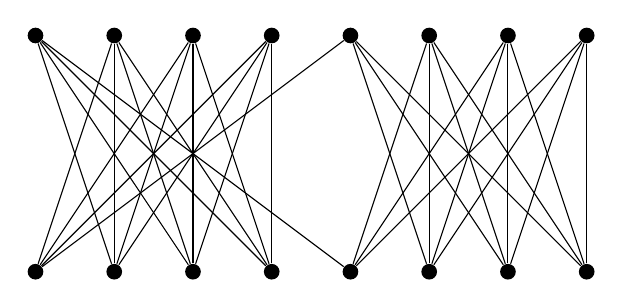
\begin{tikzpicture}[scale=1, transform shape]
          \node[circle, fill=black, inner sep=2pt] (L0) at (3.5, 0) {};
          \node[circle, fill=black, inner sep=2pt] (L1) at (2.5, 0) {};
          \node[circle, fill=black, inner sep=2pt] (L2) at (1.5, 0) {};
          \node[circle, fill=black, inner sep=2pt] (L3) at (0.5, 0) {};
          \node[circle, fill=black, inner sep=2pt] (L4) at (-0.5, 0) {};
          \node[circle, fill=black, inner sep=2pt] (L5) at (-1.5, 0) {};
          \node[circle, fill=black, inner sep=2pt] (L6) at (-2.5, 0) {};
          \node[circle, fill=black, inner sep=2pt] (L7) at (-3.5, 0) {};
          \node[circle, fill=black, inner sep=2pt] (R0) at (3.5, 3) {};
          \node[circle, fill=black, inner sep=2pt] (R1) at (2.5, 3) {};
          \node[circle, fill=black, inner sep=2pt] (R2) at (1.5, 3) {};
          \node[circle, fill=black, inner sep=2pt] (R3) at (0.5, 3) {};
          \node[circle, fill=black, inner sep=2pt] (R4) at (-0.5, 3) {};
          \node[circle, fill=black, inner sep=2pt] (R5) at (-1.5, 3) {};
          \node[circle, fill=black, inner sep=2pt] (R6) at (-2.5, 3) {};
          \node[circle, fill=black, inner sep=2pt] (R7) at (-3.5, 3) {};
          \draw (L0) -- (R0);
          \draw (L0) -- (R1);
          \draw (L0) -- (R2);
          \draw (L0) -- (R3);
          \draw (L1) -- (R0);
          \draw (L1) -- (R1);
          \draw (L1) -- (R2);
          \draw (L1) -- (R3);
          \draw (L2) -- (R0);
          \draw (L2) -- (R1);
          \draw (L2) -- (R2);
          \draw (L2) -- (R3);
          \draw (L3) -- (R0);
          \draw (L3) -- (R1);
          \draw (L3) -- (R2);
          \draw (L3) -- (R7);
          \draw (L7) -- (R3);
          \draw (L4) -- (R4);
          \draw (L4) -- (R5);
          \draw (L4) -- (R6);
          \draw (L4) -- (R7);
          \draw (L5) -- (R4);
          \draw (L5) -- (R5);
          \draw (L5) -- (R6);
          \draw (L5) -- (R7);
          \draw (L6) -- (R4);
          \draw (L6) -- (R5);
          \draw (L6) -- (R6);
          \draw (L6) -- (R7);
          \draw (L7) -- (R4);
          \draw (L7) -- (R5);
          \draw (L7) -- (R6);
        \end{tikzpicture}
    \end{figure}

    Izkaže se, da dobljeni dvig ne predstavlja Ramanujanovega grafa, zato generiramo naslednjega.
    \begin{align*}
        \begin{bmatrix}
            0 & 0 & 0 & 0 & 1 & 1 & 1 & 1 & 0 & 0 & 0 & 0 & 0 & 0 & 0 & 0\\
            0 & 0 & 0 & 0 & 1 & 1 & 1 & 1 & 0 & 0 & 0 & 0 & 0 & 0 & 0 & 0\\
            0 & 0 & 0 & 0 & 1 & 1 & 1 & 1 & 0 & 0 & 0 & 0 & 0 & 0 & 0 & 0\\
            0 & 0 & 0 & 0 & 1 & 1 & 0 & 0 & 0 & 0 & 0 & 0 & 0 & 0 & 1 & 1\\
            1 & 1 & 1 & 1 & 0 & 0 & 0 & 0 & 0 & 0 & 0 & 0 & 0 & 0 & 0 & 0\\
            1 & 1 & 1 & 1 & 0 & 0 & 0 & 0 & 0 & 0 & 0 & 0 & 0 & 0 & 0 & 0\\
            1 & 1 & 1 & 0 & 0 & 0 & 0 & 0 & 0 & 0 & 0 & 1 & 0 & 0 & 0 & 0\\
            1 & 1 & 1 & 0 & 0 & 0 & 0 & 0 & 0 & 0 & 0 & 1 & 0 & 0 & 0 & 0\\
            0 & 0 & 0 & 0 & 0 & 0 & 0 & 0 & 0 & 0 & 0 & 0 & 1 & 1 & 1 & 1\\
            0 & 0 & 0 & 0 & 0 & 0 & 0 & 0 & 0 & 0 & 0 & 0 & 1 & 1 & 1 & 1\\
            0 & 0 & 0 & 0 & 0 & 0 & 0 & 0 & 0 & 0 & 0 & 0 & 1 & 1 & 1 & 1\\
            0 & 0 & 0 & 0 & 0 & 0 & 1 & 1 & 0 & 0 & 0 & 0 & 1 & 1 & 0 & 0\\
            0 & 0 & 0 & 0 & 0 & 0 & 0 & 0 & 1 & 1 & 1 & 1 & 0 & 0 & 0 & 0\\
            0 & 0 & 0 & 0 & 0 & 0 & 0 & 0 & 1 & 1 & 1 & 1 & 0 & 0 & 0 & 0\\
            0 & 0 & 0 & 1 & 0 & 0 & 0 & 0 & 1 & 1 & 1 & 0 & 0 & 0 & 0 & 0\\
            0 & 0 & 0 & 1 & 0 & 0 & 0 & 0 & 1 & 1 & 1 & 0 & 0 & 0 & 0 & 0\\
    \end{bmatrix}
    \end{align*}
    \begin{figure}[H]
        \centering
        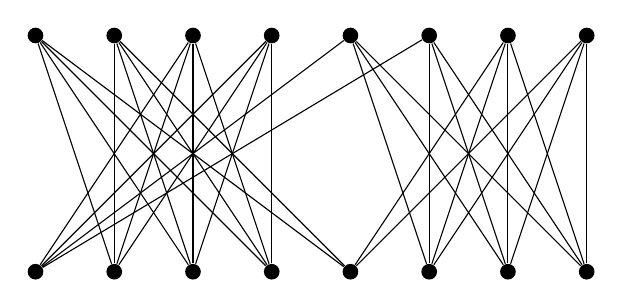
\begin{tikzpicture}[scale=1, transform shape]
          \node[circle, fill=black, inner sep=2pt] (L0) at (3.5, 0) {};
          \node[circle, fill=black, inner sep=2pt] (L1) at (2.5, 0) {};
          \node[circle, fill=black, inner sep=2pt] (L2) at (1.5, 0) {};
          \node[circle, fill=black, inner sep=2pt] (L3) at (0.5, 0) {};
          \node[circle, fill=black, inner sep=2pt] (L4) at (-0.5, 0) {};
          \node[circle, fill=black, inner sep=2pt] (L5) at (-1.5, 0) {};
          \node[circle, fill=black, inner sep=2pt] (L6) at (-2.5, 0) {};
          \node[circle, fill=black, inner sep=2pt] (L7) at (-3.5, 0) {};
          \node[circle, fill=black, inner sep=2pt] (R0) at (3.5, 3) {};
          \node[circle, fill=black, inner sep=2pt] (R1) at (2.5, 3) {};
          \node[circle, fill=black, inner sep=2pt] (R2) at (1.5, 3) {};
          \node[circle, fill=black, inner sep=2pt] (R3) at (0.5, 3) {};
          \node[circle, fill=black, inner sep=2pt] (R4) at (-0.5, 3) {};
          \node[circle, fill=black, inner sep=2pt] (R5) at (-1.5, 3) {};
          \node[circle, fill=black, inner sep=2pt] (R6) at (-2.5, 3) {};
          \node[circle, fill=black, inner sep=2pt] (R7) at (-3.5, 3) {};
          \draw (L0) -- (R0);
          \draw (L0) -- (R1);
          \draw (L0) -- (R2);
          \draw (L0) -- (R3);
          \draw (L1) -- (R0);
          \draw (L1) -- (R1);
          \draw (L1) -- (R2);
          \draw (L1) -- (R3);
          \draw (L2) -- (R0);
          \draw (L2) -- (R1);
          \draw (L2) -- (R2);
          \draw (L2) -- (R3);
          \draw (L3) -- (R0);
          \draw (L3) -- (R1);
          \draw (L3) -- (R6);
          \draw (L3) -- (R7);
          \draw (L7) -- (R2);
          \draw (L7) -- (R3);
          \draw (L4) -- (R4);
          \draw (L4) -- (R5);
          \draw (L4) -- (R6);
          \draw (L4) -- (R7);
          \draw (L5) -- (R4);
          \draw (L5) -- (R5);
          \draw (L5) -- (R6);
          \draw (L5) -- (R7);
          \draw (L6) -- (R4);
          \draw (L6) -- (R5);
          \draw (L6) -- (R6);
          \draw (L6) -- (R7);
          \draw (L7) -- (R4);
          \draw (L7) -- (R5);
        \end{tikzpicture}
    \end{figure}
    Za tega se izkaže da je Ramanujanov. Konstrukcijo od tu naprej ponavljamo induktivno in generiramo \(2\)-dvige našega novega grafa, dokler spet ne dobimo Ramanujanovega. Ker velikost dobljenih grafov raste eksponentno, postopka ne bomo nadaljevali, nam pa konstrukcija zagotavlja, da se postopek nikoli ne konča.
\end{primer}